\chapter{Development of a Particle Filter-Based Signalized Intersection Queue Estimator (PF-SIQE)}
\label{chapter: Development of a Particle Filter-Based Signalized Intersection Queue Estimator (PF-SIQE)}
This chapter presents the detailed design and operational framework of the Particle Filter-Based Signalized Intersection Queue Estimator (PF-SIQE), which is central to achieving the primary objective of this thesis: enhancing queue estimation accuracy at signalized intersections using a particle filter-based approach. Following the comprehensive literature review in Chapter \ref{chapter:Literature Review}, which analyzed existing queue estimation techniques and identified research gaps and potential advancements, this chapter details the architectural design of the PF-SIQE and provides mathematical descriptions of its core modules, as well as leveraging insights gained from previous research to inform our innovative approach. The methodology discussed herein sets the stage for Chapter \ref{chapter:Experimental Design and Analysis}, where the PF-SIQE will be subjected to rigorous simulation experiments to validate its effectiveness, test across various scenarios, and conduct sensitivity analyses to examine its robustness under different conditions. 

The initial section of this chapter introduces the fundamental structure of the PF-SIQE, comprising three primary modules: state-based prediction, measurement-based correction, and the particle filtering process. Referencing previous studies, the modularity and scalability inherent in the particle filter framework allow for the interchangeability of the prediction and correction modules with various state transition functions and measurement functions, respectively. Therefore, this chapter lays a robust groundwork for future explorations in applying particle filters to traffic state estimation or queue estimation.

The rest of this chapter methodically discusses each module of the PF-SIQE. Section \ref{Introduction to the Particle Filter Algorithm} introduces the particle filter framework, focusing specifically on how the particle filter algorithm is implemented and used in this thesis, supplemented by the provision of pseudocode. Section \ref{State Transition Function} not only describes the state transition function, which integrates a car-following model along with an acceleration/deceleration model, but also introduces acceleration noise. The acceleration/deceleration model is novel and effectively captures the complex nonlinear dynamics of human driver decision-making at the yellow light dilemma zone. This section showcases the modularity of the state-based prediction module by integrating a specific traffic flow model as a case study to demonstrate the scalability of the particle filter framework. Although integrating both longitudinal and lateral microscopic traffic flow models could better capture vehicular dynamics, this thesis includes only the longitudinal model to maintain a manageable scope, with plans to explore additional models, such as lateral movement, in future work. The state transition function establishes the ground truth for the estimations produced by the PF-SIQE. Section \ref{Measurement Function} elaborates on the measurement function, which accounts for the uncertainties associated with simulation data derived from loop detectors and connected vehicles. This section further underscores the scalability of the measurement-based correction module, noting that it is not limited to the sensors discussed herein; indeed, any point and floating sensor measurements could be integrated, providing a flexible framework for future enhancements.



\section{PF-SIQE Architecture}\label{PF-SIQE Architecture}
\begin{figure}[!htbp]
    \centering
    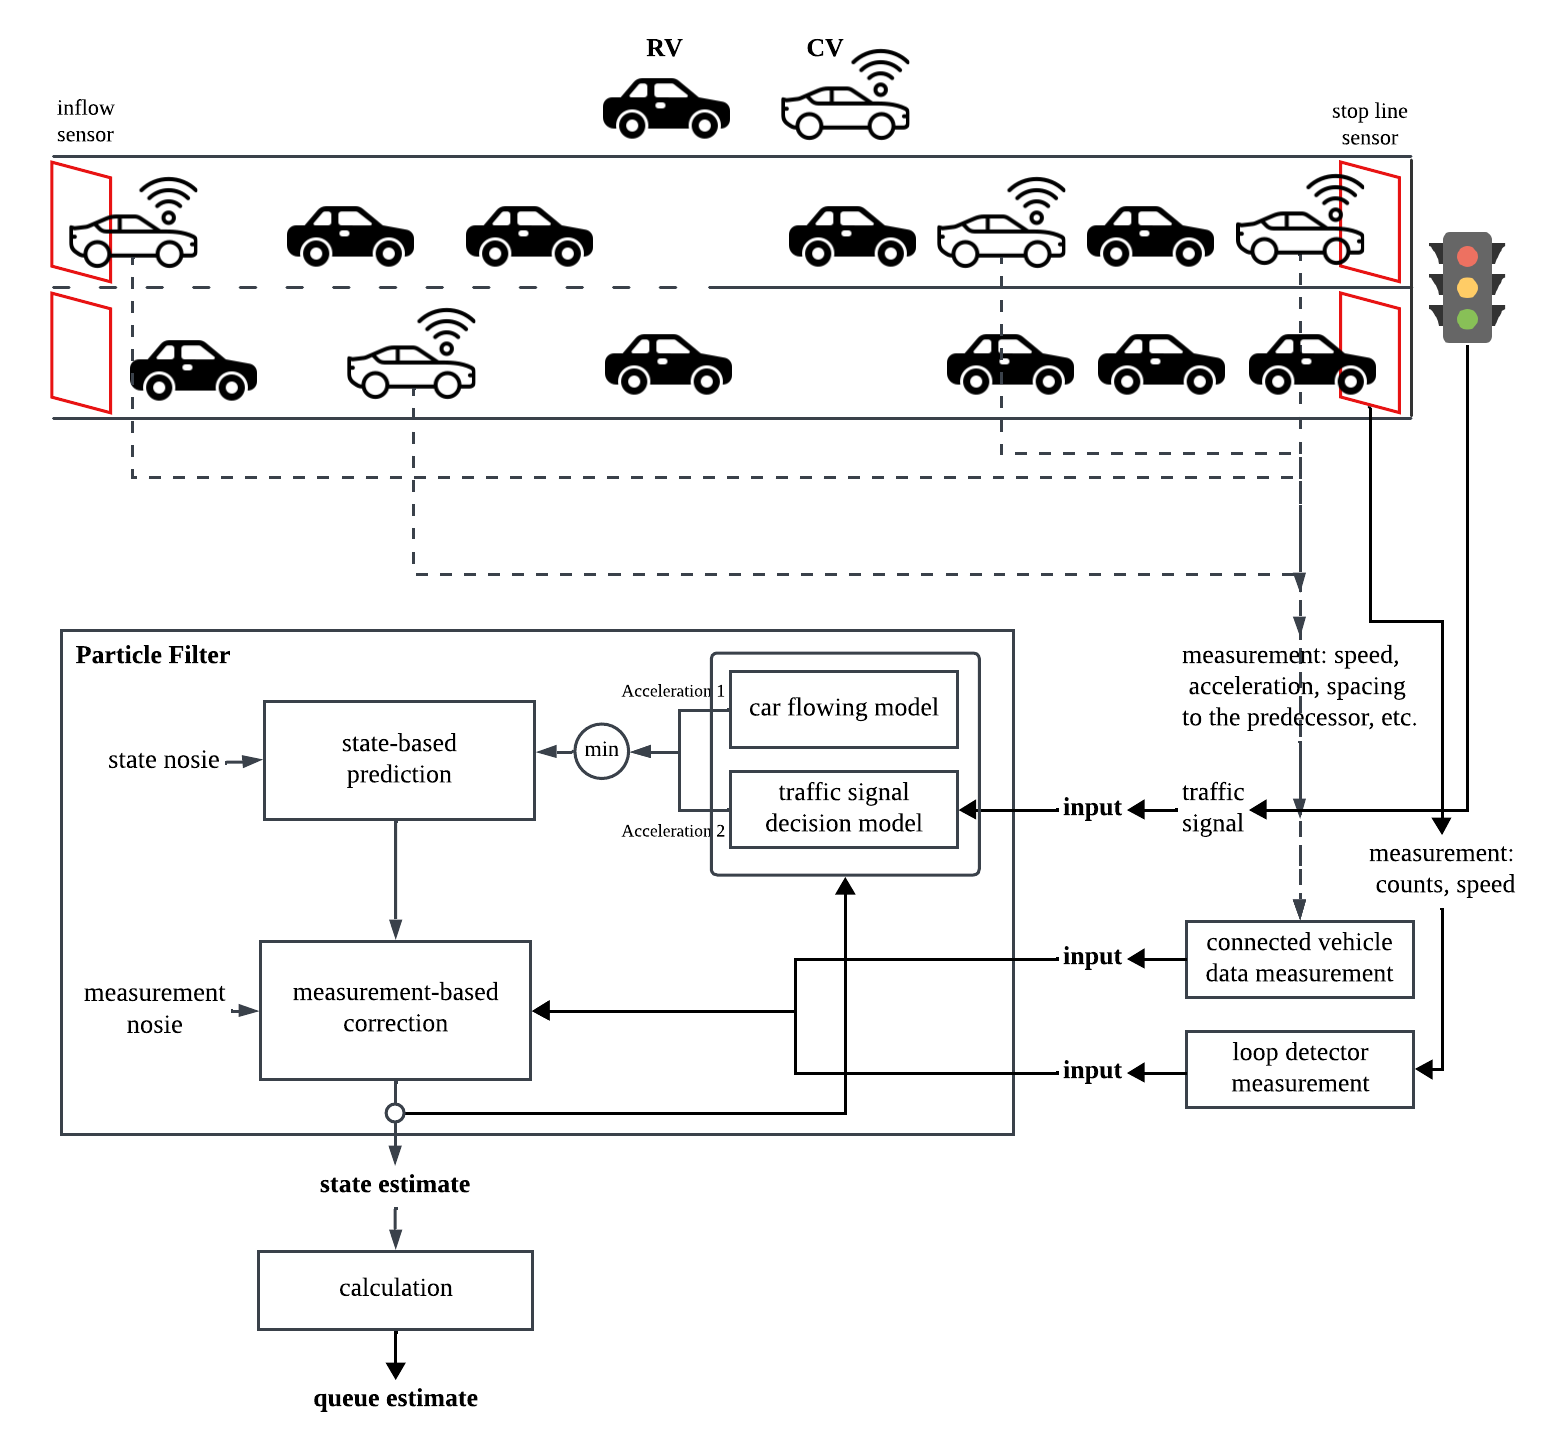
\includegraphics[width= 0.85\linewidth]{figures/architecture(1).png}
    \caption{PF-SIQE Architecture}
    \label{fig: PF-SIQE Architecture}
\end{figure}

Figure \ref{fig: PF-SIQE Architecture} illustrates the layout of a two-lane road as an example to demonstrate the particle filter framework known as PF-SIQE. This example merely explains the framework's functionality; the PF-SIQE is designed to be adaptable and applicable to various road configurations and conditions, emphasizing its generic nature and broad applicability. In this illustrative framework, connected vehicles function as floating sensors, and loop detectors act as roadside sensors to showcase the system. The framework is inherently modular, the measurement-based correction module can integrate various types of sensors beyond connected vehicles and loop detectors, highlighting its flexibility to adapt to different sensor technologies.

In this example framework, 'CV' represents connected vehicles, while 'RV' denotes regular vehicles. Assume that the CVs are equipped with GPS, providing noisy measurements at each time step, including current speed $v_k$, longitudinal distance to the stop line $d_k$, and acceleration $a_k$. LiDAR equipment on CVs measures the distance to the preceding vehicle $s_k$, as well as relative speed $\Delta v_k$ and relative acceleration $\Delta a_k$. Initially, the state transition function calculates predicted states: longitudinal position $d_{k}$, speed $v_k$, acceleration $a_k$, spacing $s_k$, lane position (lateral) $i_k^{\text{lane}}$, dilemma zone delineation ($d_a, d_b$), and decision-making processes $D_{k}$, based on previous time step prediction and the traffic signal state $S_{\text{signal}}$. These state variables are calculated by the state-based prediction module, which is one of the three principal components of the particle filter framework. To showcase the system, this module integrates the car-following model and the traffic signal decision model, both of which compute acceleration values through state transition functions. The minimum of these two acceleration values is selected and augmented with a noise term to reflect inherent system disturbances like wind resistance, road curvature, and gradients. The adjusted acceleration rate and the noise term are then used to calculate the vehicle’s speed and longitudinal position.

On the other hand, the measurement-based correction module leverages data from both the loop detector and the CVs in Figure \ref{fig: PF-SIQE Architecture}. Measurement noise is added to the data obtained from both the loop detector and the CVs. This module constructs the discrete probability function based on loop detectors' manufacturer specifications. The noise distribution in the CV measurements will be detailed in Section \ref{Measurement Function}. The joint probability is determined by taking the product of the probabilities from both data sources.

The state transition function's predictions act as the baseline for estimations. These predictions are then adjusted in a correction step through weight adjustments within the particle filter algorithm once the noisy measurements are received from CVs and additional data from loop detectors, such as vehicle counts $c_k$ and speed $v_k$.

Next, the particle filter algorithm will be introduced.


\section{Introduction to the Particle Filter Algorithm}\label{Introduction to the Particle Filter Algorithm}

The particle filter algorithm (\textcite{arulampalam2002tutorial}) is a sequential Monte Carlo method used for estimating the state of a system, where the system's state space model generates actual states, and a measurement function utilizes these measurements for correction. This section provides an overview of the key elements of the particle filter, focusing on its practical application, which sets the foundation for Section \ref{State Transition Function} and Section \ref{Measurement Function}.

\subsection{Pseudocode of the Particle Filter Algorithm}
\begin{algorithm}
\caption{Particle Filter Algorithm}\label{Particle Filter Algorithm}
\begin{algorithmic}[1]  % The [1] option enables line numbers
    \State \textbf{Input:} $\{x_{k-1}^{j}, w_{k-1}^{j}\}_{j = 1}^N, z_k$
    \State \textbf{Output:} $\{x_k^{j}, w_k^{j}\}_{j = 1}^N$
    \For{$j = 1$ \textbf{to} $N$}
        \State Draw $x_k^{j}$ from $q(x_k | x_{k-1}^{j}, z_k)$ \Comment{Typically, $q(x_k | x_{k-1}^{j}, z_k) = p(x_k | x_{k-1}^{j})$}
        \State Update weight: $\tilde{w}_k^{j} = p(z_k | x_k^{j}) w_{k-1}^{j}$
    \EndFor
    \State Normalize weights: $w_k^{j} = \frac{\tilde{w}_k^{j}}{\sum_{j=1}^N \tilde{w}_k^{j}}$
    \If{$\frac{1}{\sum_{j=1}^N (w_k^{j})^2} < N_{\text{threshold}}$}
        \State Resample particles
    \EndIf
\end{algorithmic}
\end{algorithm}
Where
\begin{itemize}
    \item $j$ is the index of the particle.
    \item $k$ is the time step.
    \item $N$ is the number of particles.
    \item $x_k^{j}$ is the state of the $j^\text{th}$ particle at time step $k$.
    \item $\tilde{w}_k^{j}$ is the intermediate weights.
    \item $w_k^{j}$ is the true weights of the new particles after the normalization process.
    \item $z_k$ is the measurement at time step $k$.
    \item $p(x_k | x_{k-1})$ is the state transition probability distribution function, which will be given in Section \ref{State Transition Probability Function}.
    \item $q(x_k | x_{k-1}^{j}, z_k)$ is the importance density function, also called the q function, when the q function is unknown, let it equal to $p(x_k | x_{k-1})$ is also a good choice typically.
    \item $p(z_k | x_k^{j})$ is the likelihood of the measurement given the state of the $j^\text{th}$ particle at time step $k$, which will be given in Section \ref{Measurement Probability Distribution Function}.
    \item $N_{\text{threshold}}$ is the threshold for the effective number of particles to decide when to resample.
\end{itemize}

In particle filters, the process of recursive estimation involves updating the particles' states and their corresponding weights based on new measurements as they become available.  The posterior distribution \( p(x_{k} | z_{1:k}) \) is approximated by a weighted set of particles \((x_{k}^{j}, w_k^{j})_{j=1}^N\), where \( \sum_{j=1}^N w_k^{j} = 1 \). Start with an initial set of particles and weights \((x_0^{j}, w_0^{j})\) at time step \(0\). When moving to the next time step, assume that the thesis knows the states and weights from the previous time step \((x_{k-1}^{j}, w_{k-1}^{j})\). The objective is to update these particles and weights to reflect the new information provided by the latest measurement \(z_k\) and the knowledge of the process dynamics.

The particle filter algorithm involves the following steps:
\begin{enumerate}
    \item Initialization: Assume the number of particles \( N \). Each particle represents a hypothetical state \( x_k \) of all the vehicles and their weight. The initial states are randomly generated, and each particle is assigned an equal weight \( w_0^{j} = \frac{1}{N} \). State $x_k$ includes various variables such as the distance to the stop line $d_k$ (longitudinal position), current speed $v_k$, acceleration $a_k$, lane position $i_k^{\text{lane}}$ (lateral position), spacing to the preceding vehicle $s_k$, dilemma zone ($d_a, d_b$), decision $D_{k}$, etc. 
    \item Prediction (Drawing Particles): The first step in the recursive estimation process is to predict the new states of the particles based on the state transition model. For each particle \(j\), a new state \(x_k^{j}\) is drawn from the importance density function \(q(x_k | x_{k-1}^{j}, z_k)\). Typically, when the exact importance density function is unknown, use the state transition probability \(p(x_k | x_{k-1})\) as an approximation. This step incorporates the system dynamics and the state noise to simulate the possible states at the new time step.
    \item Weight Update: Update the weight of each particle using the likelihood of the observed measurement \( z_k \):
      \begin{equation}
          \tilde w_k^{j} = \frac{p(z_k | x_k^{j}) p(x_k^{j} | x_{k-1}^{j})}{q(x_k | x_{k-1}^{j}, z_k)} w_{k-1}^{j}
      \end{equation}
      Since typically choose \(q(x_k | x_{k-1}^{j}, z_k) = p(x_k | x_{k-1})\), the weight update equation simplifies to:
      \begin{equation}
          \tilde w_k^{j} = p(z_k | x_k^{j}) w_{k-1}^{j}
      \end{equation}
      This means the intermediate normalized weight \(\tilde w_k^{j}\) is the product of the likelihood of the measurement \(p(z_k | x_k^{j})\) and the previous weight \(w_{k-1}^{j}\).
    \item Normalization: To ensure the weights form a valid probability distribution, they need to be normalized. This is done by dividing each weight by the sum of all weights:
      \begin{equation}
          {w}_k^{j} = \frac{\tilde w_k^{j}}{\sum_{j=1}^N \tilde w_k^{j}}
      \end{equation}
      This normalization ensures that the sum of all weights equals one.
    \item Resampling: Over time, some particles may end up with very low weights, while a few might dominate with high weights, leading to particle degeneracy. To address this, perform resampling when the effective number of particles \(N_{\text{eff}}\) falls below a certain threshold \(N_{\text{threshold}}\). The effective number of particles is estimated as:
    \begin{equation}\label{eq: effective number of particles}
        \widehat{N^{eff}} = \frac{1}{\sum_{j=1}^N ({w}_k^{j})^2}
    \end{equation}
    If \(\widehat{N^{\text{eff}}} < N_{\text{threshold}}\), resampling is triggered. In systematic resampling (see Section \ref{Systematic Resampling}), new particles are selected based on the cumulative distribution function of the normalized weights. This process ensures that particles with higher weights are more likely to be selected multiple times, while those with lower weights might be discarded. After resampling, all selected particles are assigned equal weights.
\end{enumerate}


\subsection{State Transition Probability Distribution Function: $p(x_k | x_{k-1})$}\label{State Transition Probability Function}

The state transition function \( f_k(x_{k-1}, n_{k-1}^s) \) describes how the state evolves from one time step to the next, incorporating state noise \( n_k^\text{s} \). This transition is crucial for predicting the next state based on the current state. Section \ref{State Transition Function} will present the detailed equation of $p(x_k | x_{k-1})$.

\subsection{Measurement Probability Distribution Function: $p(z_k | x_k^{j})$}\label{Measurement Probability Distribution Function}

The measurement function \( g_k(x_k, n_k^\text{m}) \) incorporates measurement noise \( n_k^\text{m} \) and provides the likelihood of the observed measurement given the state. This likelihood function \( p(z_k | x_k) \) is essential for updating the weights of the particles, which will be presented in Section \ref{Measurement Function}.

\subsection{Importance Density Function (q-function): \textbf{$q(x_k | x_{k-1}^{j}, z_k)$}}\label{q function}

In particle filters, selecting the importance density function \( q(x_k | x_{k-1}, z_k) \) is critical for drawing new particles. A common and practical choice is the state transition function \( p(x_k | x_{k-1}) \). This selection simplifies the weight update process and is the approach adopted in this thesis.

\subsection{Systematic Resampling}\label{Systematic Resampling}

Systematic resampling is a method used in particle filters to address the issue of particle degeneracy, where over time, a few particles may carry the majority of the weight, reducing the diversity of the particle set. This resampling method ensures that particles with higher weights are more likely to be selected, while particles with lower weights are less likely to survive, thereby maintaining a diverse and representative set of particles.

Here are the steps of systematic resampling:
\begin{enumerate}
    \item Compute the Cumulative Sum of Weights: Begin by computing the cumulative sum of the normalized weights of the particles. This step forms a cumulative distribution function (CDF) that will be used to draw particles for the next iteration. Essentially, you sum the weights sequentially so that each particle’s weight is added to the sum of all previous weights.
    \item Initialize Variables:
    \begin{itemize}
        \item Generate a random starting point, which is a random number uniformly distributed between 0 and the reciprocal of the number of particles ($\frac{1}{N}$). This random starting point ensures that the particles are resampled in a systematic but random manner.
        \item Set the initial index to 1. This index will be used to track which particle is being selected during the resampling process.
    \end{itemize}
    \item Resample Particles:
    \begin{itemize}
        \item For each particle in the set, calculate a target value by adding a fixed step size to the initial random starting point. The step size is the reciprocal of the number of particles ($\frac{1}{N}$).
        \item Move through the cumulative sum of weights and select particles based on the target values. If the target value falls within the cumulative weight range of a particle, that particle is selected.
        \item Assign the state of the selected particle to a new set of particles, ensuring that particles with higher weights (which have larger cumulative sums) are more likely to be chosen.
        \item After selecting a particle, assign it an equal weight, so all particles in the new set start with the same weight.
    \end{itemize}
    \item Stop Criterion: The resampling process is completed once all $N$ particles have been resampled. This is guaranteed after exactly $N$ iterations, as each iteration selects one particle based on the target values and cumulative sum of weights. Thus, the resampling process stops when the full set of $N$ particles has been replaced in the new particle set.
\end{enumerate}



Following this introduction to the particle filter algorithm, the subsequent sections will present details on the state transition function, state noise distribution, measurement function, and measurement noise distribution, with a focus on their practical implementation within the proposed framework.


\section{State Transition Function Module}\label{State Transition Function}
To align with the research objective, the particle filter will provide as accurate as possible queue estimations despite state noise and measurement noise. In the particle filter framework, the state transition function's predictions act as the baseline for estimations. These predictions are then adjusted in a correction step through weight adjustments within the particle filter algorithm once the noisy measurements are received from sensors.

When considering which state variables to include, they should align with the models that the state transition function module aims to integrate. This alignment ensures consistency and coherence between the state variables and the models used to describe the system dynamics. To maintain the scalability and align with the research objective, the state transition function in the thesis considers a wide range of state variables of the vehicles to represent the system: 
\begin{equation}\label{state variables}
    x_k^i = \begin{bmatrix}
d_k^i & v_k^i & a_k^i  & D_{k}^i & i_k^{\text{lane}}
\end{bmatrix}
\end{equation}

where
\begin{itemize}
    \item $k$ is the time step index.
    \item $i$ is the vehicle index. Keep the direction intuitive, from upstream to downstream.
    \item $x_k^i$ is the system state for one vehicle. 
    \item $d_k^i$ [m] is the longitudinal position of the  $i^{th}$ vehicle along the road. Keep the direction intuitive, from upstream to downstream.
    \item $v_k^i$ [m/s] is the instantaneous speed.
    \item $a_k^i$ [m/s$^2$] is the instantaneous acceleration rate.
    \item $D_{k}^i$ is the decision of stop or go when facing the traffic light.
    \item $i_k^{\text{lane}}$ is the index number of which lane the vehicle is.
    %\item $s_k$ [m] is the current gap to the predecessor.
    %\item $d_a$ [m] is the downstream boundary of the dilemma zone.
    %\item $d_b$ [m] is the upstream boundary of the dilemma zone.
\end{itemize}

\subsection{Handling Multiple Vehicles}
To cope with multiple vehicles, the system state vector \( X_k \) is extended to include the state vectors of all vehicles in a selected road segment at each time step $k$:
\begin{equation}
    X_k = \begin{bmatrix}
x_k^1 \\
x_k^2 \\
\cdots \\
x_k^N 
\end{bmatrix}
= \begin{bmatrix}
d_k^1 & v_k^1 & a_k^1 & D_{k}^1 & i_k^{\text{lane}, 1}  \\
d_k^2 & v_k^2 & a_k^2 & D_{k}^2 & i_k^{\text{lane}, 2}  \\
\text{$\cdot \cdot \cdot $} \\
d_k^N & v_k^N & a_k^N & D_{k}^N & i_k^{\text{lane}, N}  \\
\end{bmatrix}
\end{equation}

where \( N \) is the total number of vehicles within a specific road segment. The thesis assumes that the total number of vehicles \( N \) is constant during the estimation process within a certain time period for a given road segment. This assumption simplifies the model by not considering vehicle arrival or departure patterns. Future work could integrate vehicle arrival distributions and departure processes for more dynamic modeling, as discussed in the final chapter.





\subsection{State Transition Function}
The state transition function describes how these state variables evolve from one time step to the next, incorporating the system's dynamics, the influence of control inputs, and the presence of noise. The state transition function expresses:

\begin{enumerate}
    \item Calculation of All States: The function provides a mathematical description of how each state variable is updated at each time step.
    \item Introduction of the State Noise Term: The function incorporates state noise \(n_k^\text{s}\) to account for the randomness and uncertainties in the system dynamics.
    \item State Probability Distribution Function: The function defines the probability distribution function \(p(x_k | x_{k-1})\), which describes the likelihood of transitioning from one state to another.
\end{enumerate}

\begin{equation}
    x_{k+1} = f(x_k, n_k^\text{s}) 
\end{equation}
\begin{equation}
    d_{k+1} = d_k + v_k \cdot T + \frac{1}{2} \cdot a_k \cdot T^2  +  n_k^\text{s}  
\end{equation}
\begin{equation}
    v_{k+1} = v_k +  a_k \cdot T +  n_k^\text{s}  
\end{equation}
\begin{equation}
    a_{k+1} = \min (\bar a_{k+1}, \tilde a_{k+1}) +  n_k^\text{s}  
\end{equation}
\begin{equation}
    i_{k+1}^{\text{lane}} = g(x_k, \text{lane change external factors})
\end{equation}

where
\begin{itemize}
    \item $T$ [s] is the time step, in the simulation detailed in Chapter \ref{chapter:Experimental Design and Analysis}, $T$ is set to 1 second.
    \item $n_k^\text{s}$ is the state noise term. In this thesis, $n_k^\text{s}$ indicates the randomness $n_k^\text{d}$ in the decision-making process and the acceleration noise $n_k^\text{a}$, which will be detailed in Section \ref{State noise distribution}.
    \item $\bar a_{k+1}$ [m/s$^2$] is the acceleration rate involving the car-following model, detailed in Section \ref{car-following model: IDM}.
    \item $\tilde a_{k+1}$ [m/s$^2$] is the acceleration rate involving traffic signal status, detailed in Section \ref{Longitudinal}.
    %\item $f(a_{\text{max}}, v_k, v_{\text{desired}}, \delta, \Delta v_k, s_0, h_s, b, s_k, d_a, d_b, S_{\text{signal}}, D_{k})$ is a function that updates the acceleration based on current acceleration and external factors such as the distance to the predecessor, traffic signal status, etc. This will be addressed in the next Section \ref{Longitudinal}.
    \item $g(x_k, \text{lane change external factors})$ is a function that updates the lane position based on the current lane position and any lane change external factors, such as the surrounding vehicles, the road layout, lane change intention, or the route information.
    %\item The calculation of $s_k,  d_a,  d_b,  D_{k}$ is presented in Section \ref{Longitudinal}.
\end{itemize}
The process will occur in two phases: initially, the car-following and traffic signal decision models (so-called traffic light acceleration/deceleration models) will be applied to update the longitudinal state as a vehicle approaches a traffic signal. In future work, the lane change model may be incorporated to accurately represent lateral movements, enhancing the realism of the vehicle's behavior at intersections.


\subsection{Phase 1: Longitudinal Motion}\label{Longitudinal}
Given that the PF-SIQE primarily targets queue estimation near traffic signals, it is crucial to consider vehicle behavior (i.e. acceleration or deceleration) in response to the predecessor as well as the traffic signals when approaching and exiting the intersection. The particle filter framework is highly versatile and capable of integrating a variety of models, not limited to microscopic traffic flow models. To illustrate this versatility, this section presents the mathematical description of the integration of the car-following model and the traffic signal decision model and focuses on the calculation of $a_{k+1} = \min (\bar a_{k+1}, \tilde a_{k+1}) +  n_k^\text{s}$. The Intelligent Driver Model (IDM) from \textcite{treiber2000congested} is chosen as the car-following model in this thesis to capture the dynamic between vehicles longitudinally. Meanwhile, the traffic signal decision model is modified based on the bike acceleration/deceleration model presented by \textcite{dabiri2020optimized} to simulate the driver's response to the traffic signal. These models will be implemented in Chapter \ref{chapter:Experimental Design and Analysis} Experimental Simulation to demonstrate their effectiveness within the PF-SIQE framework.


\subsubsection{Car-Following Model: Intelligent Driver Model (IDM)}\label{car-following model: IDM}

\begin{table}[htbp]
\small
    \centering
    \begin{tabular}{cccccc}
    \toprule
         & desired  & maximum   & comfortable   & minimum   & safe time   \\
         name & speed  &  acceleration  &  deceleration  &  gap  &  headway  \\
         & \(v_{\text{desired}}\) (m/s) & $a_{\text{max}}$ (m/s$^2$)& $b$ (m/s$^2$) & $s_0$ (m) & $h_s$ (s) \\
        \hline
         value & 15.0 & 1.0 & 1.5 & 2.0 & 1.0 \\
         \toprule
    \end{tabular}
    \caption{The parameters of IDM (\textcite{treiber2013traffic})}
    \label{parameters of IDM}
\end{table}


There are plenty of car-following models developed in the previous studies. Note that the state transition function module is flexible and versatile to replace any other car-following models or lane change models with the chosen one in this thesis. \textcite{treiber2000congested} presented the Intelligent driver model(IDM), which calculates the current acceleration \(a\) by multiplying \(a_{\text{max}}\) with an adjustment factor. This adjustment factor takes into account the desired speed $v_{\text{desired}}$, the current speed $v_k$, and the current gap to the predecessor $s_k$, to simulate the driver's response to the predecessor:

\begin{equation}\label{acceleration update equation 1}
     \bar a_{k+1}  = a_{\text{max}} \left( 1 - \left( \frac{v_k}{v_{\text{desired}}} \right)^\delta - \left( \frac{s_k^*(v_k, \Delta v_k)}{s_k} \right)^2 \right) 
     %f(a_{\text{max}}, v_k, v_{\text{desired}}, \delta, \Delta v_k, s_0, h_s, b, s_k)
\end{equation}
where
\begin{itemize}
    \item \(\bar a_{k+1}\) [m/s$^2$] represents the vehicle's acceleration at time step $k+1$.
    \item \(a_{\text{max}}\) [m/s$^2$] is a model parameter that represents the maximum acceleration a vehicle can achieve under ideal conditions, reflecting the vehicle's ability to accelerate from a stationary state to its top speed.
    \item \(v_k\) [m/s] is the current speed.
    \item \(v_{\text{desired}}\) [m/s] is the desired speed, which in this case refers to the speed limit of the road segment, and is set as a model parameter. Although individual drivers may have different desired speeds, the IDM model assumes that all drivers aim to reach the maximum allowable speed, i.e., the speed limit of the road, as a simplifying assumption in this study.
    \item \(\delta\) is the free flow exponent, typically set to 4.
    \item \(s_k\) [m] is the current gap of the $i^\text{th}$ vehicle to the predecessor ${(i-1)}^\text{th}$, which can be calculated as:
    \begin{equation}
        s_k^i = d_k^{i-1} - d_k^i - l^{i-1}
    \end{equation}
    where $l^{i-1}$ is the vehicle length of the predecessor.
    \item \(\Delta v_k\) [m/s] is the relative speed to the predecessor:
    \begin{equation}
        \Delta v_k = v_k^{i} - v_k^{i-1}
    \end{equation}
    \item \(s_k^*(v_k, \Delta v_k)\) [m] denotes the desired gap, also referred to as the dynamic following distance, written as:
    \begin{equation}
    s_k^*(v_k, \Delta v_k) = s_0 + v_k h_s + \frac{v_k\Delta v_k}{2\sqrt{a_{\text{max}}b}}
    \end{equation}
    where:
    \begin{itemize}
        \item \(s_0\) [m] is the minimum gap when vehicles are stationary to ensure that collisions do not occur in a standstill situation. The specific value of \(s_0\) can be set according to the type of vehicle, traffic regulations, or driving behaviors. For instance, in some models, \(s_0\) can be set to approximately 2 m.
        \item \(h_s\) [s] refers to the safe time headway a driver wishes to maintain between themselves and the predecessor while following. In practice, \(h_s\) is often set to a value between 1 s and 2 s, to simulate driving behavior under most road conditions.
        \item \(b\) [m/s$^2$] is the comfortable deceleration rate, indicating the desired deceleration when slowing down. The value of \(b\) ranges between 1.5 to 3.0 m/s$^2$.
    \end{itemize}
\end{itemize}

Table \ref{parameters of IDM} shows the parameters of IDM. The desired speed $v_{\text{desired}} = 15 \text{ m/s}$ aligns with the common speed limit in urban areas, which is $50$ km/h. The justifications for the other parameters can be found in \textcite{treiber2013traffic}.

In the absence of a predecessor (\(s_k \rightarrow \infty\)), the acceleration for next time step \(\bar a_{k+1}\) attempts to bring the vehicle to its desired speed \(v_{\text{desired}}\). When a predecessor is present, the acceleration is influenced by two factors: the desire to reach the desired speed and the need to maintain a safe distance from the predecessor. The \(s_k^*(v_k, \Delta v_k)\) function considers the current speed, the speed difference with the predecessor, and the acceleration needed to decelerate within a safe distance, ensuring that the vehicle maintains smooth traffic flow while being capable of decelerating safely when necessary.





\subsubsection{Traffic Signal Decision Model: Acceleration/Deceleration Model}\label{Traffic Signal Decision Model: Acceleration/Deceleration Model}

Adopting a vehicle-based perspective aligns with the particle filter algorithm, shifting focus from traditional management to individual vehicle control. This approach assumes that each vehicle, whether connected or not, makes decisions based on crucial parameters such as speed limits, yellow light duration, dilemma zone boundary, reaction times, deceleration rates, and the current speed. Consequently, each vehicle can determine its position relative to its dilemma zone, whether it is approaching, within, or past it. If the traffic signal is yellow, vehicles upstream of its dilemma zone will stop, those within its dilemma zone will make a decision to stop or go (modeled as a probabilistic decision), and vehicles downstream of its dilemma zone will continue to go. This model ensures that the particle filter framework accurately represents the decision-making process for all vehicles at traffic signals, enhancing the overall realism and effectiveness of the queue estimation process.

In the context of the vehicle and traffic signal interaction, the essence of our investigation centers on how vehicles autonomously respond to traffic light changes. Emphasizing the vehicle's decision-making at traffic signals, the thesis explores the decisive moments and criteria for choosing to either stop or proceed. This analysis begins by establishing the decision-making boundary where vehicles must instantaneously respond to traffic signals, adhering to their chosen course of action.

Deciding whether to stop or go is straightforward when the traffic signal is green or red (see the decision-making model Equation \ref{decision}), but it becomes challenging when the signal is yellow. The concept of the vehicle's dilemma zone is critical in this framework, signifying a region of uncertainty faced by vehicles at a yellow light. Decision-making in this zone is influenced by several factors, including the vehicle's speed and proximity to the intersection, which dictate whether stopping or continuing is the safer option.

First, introduce the physical decision-making boundary on the road segment $D_h$: 
\begin{itemize}
    \item $D_h$ indicates the distance at which a driver begins to respond to the traffic signal, marking the initiation point for decision-making regarding the signal status.
    \item Assume the traffic signal is visible within \(D_h\). 
    \item It is assumed that once a decision is reached within the dilemma zone, it is adhered to without deviation.
    %\item Reference for brake response times for the 'first-to-stop' vehicles is made to \cite{gates2007analysis}, detailing observed 15th, 50th, and 85th percentile brake-response times as 0.7, 1.0, and 1.6 seconds, respectively.
\end{itemize}


\begin{figure}[!htbp]
    \centering
    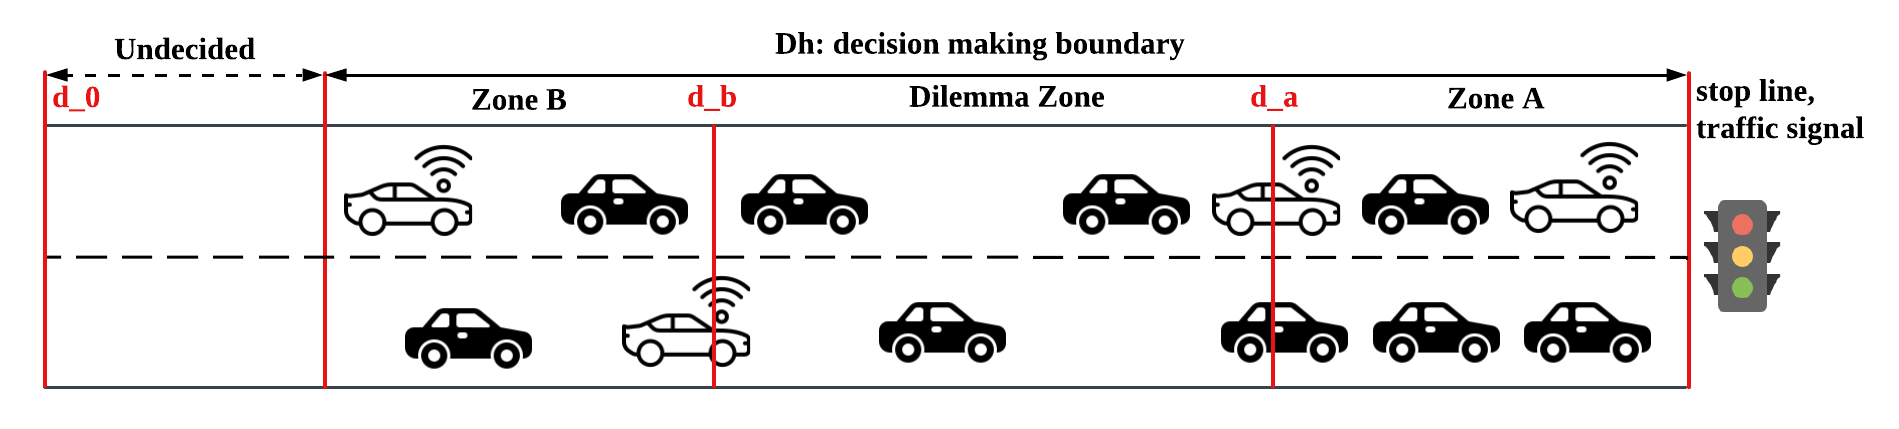
\includegraphics[width= 0.85\linewidth]{figures/dilemma zone1.png}
    \caption{Dilemma Zone}
    \label{fig: Dilemma Zone}
\end{figure}

\begin{table}[htp]
\small
    \centering
    \begin{tabular}{ccccc}
    \toprule
         &    reaction   &  deceleration   & yellow   & comfortable   \\
        name &  time  &   rate  &  time  &  acceleration  \\
         &  $T_{\text{reaction}}$ (s)& $b$ (m/s$^2$) & $T_{\text{yellow}}$ (s) & $a'$ (m/s$^2$) \\
        \hline
         value & 1.0 & 1.0 & 3.5 & 1.0 \\
         \toprule
    \end{tabular}
    \caption{The parameters of traffic signal decision model (\textcite{gates2007analysis})}
    \label{parameters of traffic signal decision model }
\end{table}
Table \ref{parameters of traffic signal decision model } shows the recommended value of the parameters in the traffic signal decision model. The justification could be found in \textcite{gates2007analysis}.

Then, present the downstream boundary $d_a$ of the vehicle's dilemma zone:

As illustrated in Figure \ref{fig: Dilemma Zone}, a vehicle requires a minimum braking distance to halt fully and securely at the stop line. This minimum braking distance defines the downstream boundary of the vehicle's dilemma zone, indicating that failing to initiate braking at this point eliminates the possibility of stopping safely and comfortably before reaching the stop line. Assume that the road gradient at the study intersection is zero (\textcite{gates2007analysis}, see equation 1),
\begin{equation}\label{downstream boundary}
    d_{a, k} = T_{\text{reaction}}v_k + \frac{v_k^2}{2b}
\end{equation}
where
\begin{itemize}
    \item $T_{\text{reaction}}$ [s] is the brake reaction time, recommended 1.0 s.
    \item $v_k$ [m/s] is the current speed.
    \item $b$ [m/s$^2$] is the deceleration rate, recommended -3.0 m/s$^2$.
\end{itemize}


Next, introduce the upstream boundary $d_b$ of the vehicle's dilemma zone:

The dilemma zone's upstream boundary indicates the location from which the stop line can just be reached if the vehicle's speed remains unchanged from the remaining time of the yellow signal to the end of the yellow signal,
\begin{equation}\label{upstream boundary}
    d_{b, k} = T_kv_k 
\end{equation}
where
\begin{itemize}
    \item $T_{\text{yellow}}$ [s] is the total yellow time, recommended 3.5 s.
    \item $T_k$ [s] is the remaining time of the yellow signal. Assume that the vehicle knows the remaining yellow time:
    \begin{equation}\label{remaining yellow time}
        T_k = T_{\text{yellow}} - T_{\text{elapsed}, k}
    \end{equation}
\end{itemize}

Deciding to go or stop is quite straightforward when the traffic light is green or red. However, the challenge arises with a yellow light. When facing a yellow light, there may be two distinct dilemma zones:
\begin{itemize}
    \item Two Options Dilemma Zone: This is the segment between \( d_a \) and \( d_b \). The downstream boundary \( d_a \) is determined by the braking distance, current speed, and deceleration rate, while the upstream boundary \( d_b \) is determined by the desired speed and the remaining yellow time. Within this dilemma zone, a vehicle could choose to stop or go, both of which are feasible options. The presence of this dilemma zone can cause confusion, especially if two longitudinally adjacent vehicles make different decisions (e.g., the predecessor chooses to stop while the successor chooses to go), creating a potential risk of collision. Therefore, modeling the randomness during the decision-making process within this two options dilemma zone is necessary.
    %\item Pitfall Zone: This is the area extending from the stop line to \( d_a \), where it is not possible to pass or stop safely. In this zone, the yellow time is too short to allow the vehicle to pass successfully at the desired speed, and the distance to the stop line is too short for a safe braking maneuver, making it impossible to stop comfortably before the stop line. This thesis assumes that the yellow time is long enough to avoid the pitfall zone.
    \item Pitfall Zone: This is the area extending between \(d_a\) and \(d_b\) when \(d_a\) is upstream of \(d_b\). In this zone, the yellow time is too short to allow the vehicle to pass successfully at the desired speed, and the distance to the stop line is too short for a safe braking maneuver, making it impossible to stop comfortably before the stop line. If \(d_b\) is more upstream, the pitfall zone extends between \(d_a\) and the stop line, where the vehicle cannot stop safely and should continue through the intersection. This thesis assumes that the yellow time is long enough to avoid the pitfall zone.
\end{itemize}

\begin{figure}[!htbp]
    \centering
    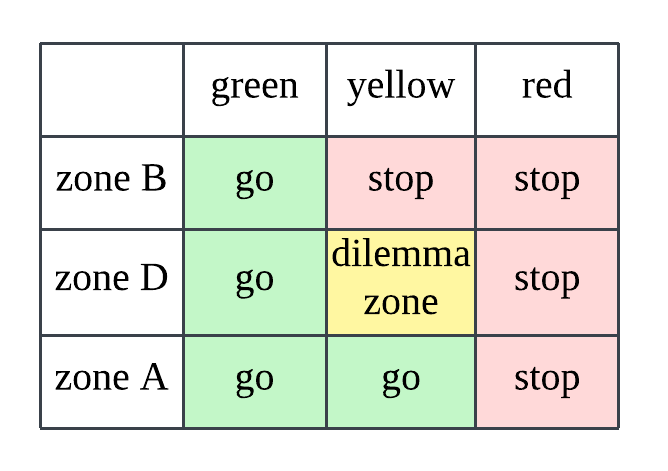
\includegraphics[width= 0.45\linewidth]{figures/decision making.png}
    \caption{Decision making}
    \label{fig: Decision making}
\end{figure}
\begin{figure}[!htbp]
    \centering
    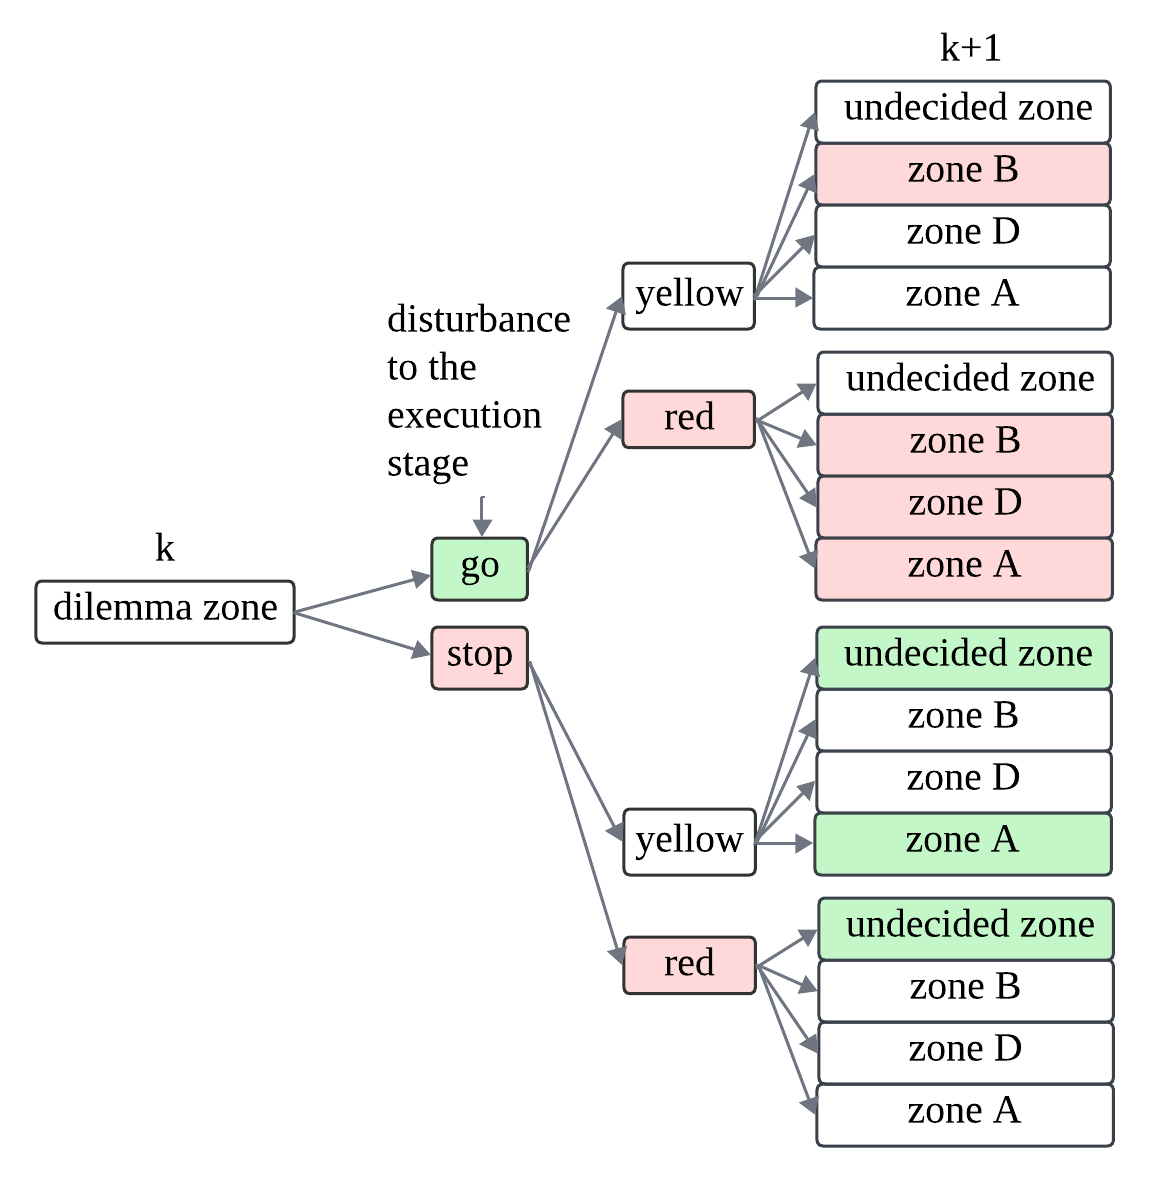
\includegraphics[width= 0.65\linewidth]{figures/decision making for dilemma zone.png}
    \caption{Decision making for dilemma zone: conflicting between $k$ and $k+1$}
    \label{fig: Decision making for dilemma zone}
\end{figure}



In Figure \ref{fig: Dilemma Zone}, Zone A is defined as the area extending from $d_a$ to the stop line $d_\text{stop line}$. Consequently, a driver has to proceed if they are in zone A when encountering a yellow light. The segment between $d_b$ and $d_a$ denotes the Two Options Dilemma Zone, where drivers are faced with the decision to either continue or halt based on a predefined probability distribution. Zone B stretches from $D_h$ to $d_b$, indicating a region where the default action for drivers is to stop. In summary, when a vehicle approaches from upstream of the traffic signal (Figure \ref{fig: Decision making}):
\begin{itemize}
    \item If the signal status is red ($S_{k+1} = S_{\text{red}}$), the decision is to stop, $D_{k+1} = D_{\text{stop}}$.
    \item If the signal status is green ($S_{k+1} = S_{\text{green}}$), the decision is to maintain speed according to the car-following model, $D_{k+1} = D_{\text{go}}$.
    \item If the signal status is yellow ($S_{k+1} = S_{\text{yellow}}$):
    \begin{itemize}
        \item If the vehicle is in Zone B ($D_h \leq d_{k+1} \leq d_{b, k+1}$), the decision is to stop, $D_{k+1} = D_{\text{stop}}$.
        \item If the vehicle is in Zone A ($d_{a, k+1} \leq d_{k+1} \leq d_\text{stop line}$), the decision is to proceed, $D_{k+1} = D_{\text{go}}$. 
        \item Figure \ref{fig: Decision making for dilemma zone} illustrates the exceptions to adhering to decisions within the dilemma zone. For instance, if a vehicle is within its dilemma zone and decides to proceed at time step \(k\), it might face disturbances during the execution stage, such as the predecessor slowing down. Consequently, at \(k+1\), if the traffic signal remains yellow, the vehicle might end up in Zone B. According to Figure \ref{fig: Decision making}, in the (yellow, Zone B) scenario, the decision should be to stop. Therefore,
        \begin{itemize}
            \item If both at time step $k$ and $k+1$, the vehicle is within its dilemma zone, particles will adhere to a probability distribution to either pass or stop and once decided, the vehicle will stick to this decision.
            \item If at time step $k$ the vehicle is within its dilemma zone, while at time step $k+1$ the vehicle is not within the dilemma zone, the vehicle will not stick to the decision at time step $k$.
            \item In conclusion, if and only if both at time step $k$ and $k+1$, the vehicle is within its dilemma zone, the vehicle will stick to the decision.
        \end{itemize}
    \end{itemize} 
\end{itemize}

For the dilemma zone, introduce a discrete probability distribution to model the vehicle's decision-making process in its dilemma zone. Define the probability of stopping as follows:

\begin{equation}
    p(D_{\text{stop}} | S_{\text{yellow}}, D_\text{undecided}, d_{b, k+1} < d_{k+1} < d_{a, k+1}) = p
\end{equation}

Thus, the probability of going is:

\begin{equation}
    p(D_{\text{go}} | S_{\text{yellow}}, D_\text{undecided}, d_{b, k+1} < d_{k+1} < d_{a, k+1}) = 1 - p
\end{equation}

where:
\begin{itemize}
    \item \(p\) is the probability that the vehicle chooses to stop when facing a yellow light in its dilemma zone.
\end{itemize}

Therefore, the decision $D_{k+1}^i$ of the $i^{th}$ individual vehicle responding to the signal status can be defined as a state-space model:
\begin{equation}\label{decision}
    D_{k+1}^i = 
\begin{cases} 
D_{\text{undecided}}, & \text{if } d_0 \leq d_{k+1} \leq D_h \text{ (undecided zone) },\\
D_{\text{stop}}, &  \begin{cases}
    \text{if } D_h \leq d_{k+1} \leq d_\text{stop line} \text{ (decided zone)}, S_{k+1} = S_{\text{red}}, \\
    \text{if } D_h \leq d_{k+1} \leq d_{b, k+1} \text{ (zone B)}, S_{k+1} = S_{\text{yellow}}, \\
    \text{if } d_{b, k+1} < d_{k+1} < d_{a, k+1} \text{ (dilemma zone)}, S_{k+1} = S_{\text{yellow}}, \\D_k = D_\text{undecided} \text{ or } d_k \text{ is out of dilemma zone},\text{and } p_\text{stop} = p, \\
\end{cases} \\
D_{\text{go}}, & \begin{cases}
    \text{if } D_h \leq d_{k+1} \leq d_\text{stop line} \text{ (decided zone)}, S_{k+1} = S_{\text{green}}, \\
    \text{if } d_{a, k+1} \leq d_{k+1} \leq d_\text{stop line} \text{ (zone A)}, S_{k+1} = S_{\text{yellow}}, \\
    \text{if } d_{b, k+1} < d_{k+1} < d_{a, k+1} \text{ (dilemma zone)}, S_{k+1} = S_{\text{yellow}}, \\D_k = D_\text{undecided}\text{ or } d_k \text{ is out of dilemma zone}, \text{and } p_\text{go} = 1 - p, \\
\end{cases} \\
D_{k}^i, & \text{if and only if both at time step $k$ and $k+1$, the vehicle is within its dilemma zone}.
\end{cases}
\end{equation}
First, during initialization, when the vehicle approaches from upstream towards the traffic signal and \(d_0 \leq d_{k+1} \leq D_h\), the initial decision has not yet been made, denoted as \(D_{k+1} = D_{\text{undecided}}\). The state \(D_{\text{undecided}}\) ensures that the vehicle can dynamically update its decision based on the signal status and its position relative to its dilemma zone. Once the decision is made at time step $k$, the vehicle will adhere to this decision in subsequent time steps, meaning $D_{k+1}^i = D_{k}^i$ if the decision has already been made at the time step $k$. This state-space model allows the decision-making process to be dynamically updated based on the vehicle's previous decision and the current signal status, ensuring consistency in the vehicle's behavior once a decision has been made.

Here is the pseudocode for the decision-making process of vehicles at traffic signals: Algorithm \ref{Traffic Signal Decision-Making Algorithm}.
\begin{algorithm}[htp]
\caption{Traffic Signal Decision-Making Algorithm}\label{Traffic Signal Decision-Making Algorithm}
\begin{algorithmic}[1]  % The [1] option enables line numbers
    \State \textbf{Input:} $d_k^i, d_{k+1}^i, v_k^i, v_{k+1}^i, S_k, S_{k+1}, T_k^i, T_{k+1}^i, D_k^i, p$
    \State \textbf{Output:} $D_{k+1}^i$
    \State \textbf{Constants:} $D_h = 150$, $T_{\text{reaction}} = 1.0$, $b = 3.0$, $T_{\text{yellow}} = 3.5$
    \For{$i = 1$ \textbf{to} $N$}
        \If{$d_0 \leq d_{k+1}^i \leq D_h$}
            \State $D_{k+1}^i = D_{\text{undecided}}$
        \Else
            \If{$S_{k+1} = S_{\text{red}}$}
                \If{$D_h \leq d_{k+1}^i \leq d_\text{stop line}$}
                    \State $D_{k+1}^i = D_{\text{stop}}$
                \EndIf
            \ElsIf{$S_{k+1} = S_{\text{green}}$}
                \If{$D_h \leq d_{k+1}^i \leq d_\text{stop line}$}
                    \State $D_{k+1}^i = D_{\text{go}}$
                \EndIf
            \ElsIf{$S_{k+1} = S_{\text{yellow}}$}
                \State Calculate downstream boundary $d_{a, k+1}^i = T_{\text{reaction}} \cdot v_{k+1}^i + \frac{(v_{k+1}^i)^2}{2 \cdot b}$
                \State Calculate remaining yellow time $T_{k+1}^i = T_{\text{yellow}} -T_{\text{elapsed}, {k+1}}^i$
                \State Calculate upstream boundary $d_{b, k+1}^i = T_{k+1}^i \cdot v_{k+1}^i$
                \If{$D_h \leq d_{k+1}^i \leq d_{b, k+1}^i$}
                    \State $D_{k+1}^i = D_{\text{stop}}$
                \ElsIf{$d_{a, k+1}^i \leq d_{k+1}^i \leq d_\text{stop line}$}
                    \State $D_{k+1}^i = D_{\text{go}}$
                \ElsIf{$d_{b, k+1}^i < d_{k+1}^i < d_{a, k+1}^i$}
                \State Calculate boundaries at time step $k: d_{b, k}^i, d_{a, k}^i$
                    \If{$d_{a, k}^i \leq d_k^i, d_k^i \leq d_{b, k}^i$ \textbf{or} $D_k^i = D_{\text{undecided}}$} 
                        \State Generate a random value $r \sim \mathcal{U}[0, 1]$
                        \If{$r < p$}
                            \State $D_{k+1}^i = D_{\text{stop}}$
                        \Else
                            \State $D_{k+1}^i = D_{\text{go}}$
                        \EndIf
                    \EndIf
                \EndIf
            \EndIf
        \EndIf
        \If{$S_k = S_{k+1} = S_{\text{yellow}}$ \textbf{and} $D_{k}^i = D_{\text{decided}}$}
            \State Calculate boundaries at $k$ and $k+1$: $d_{b, k}^i, d_{a, k}^i, d_{b, k+1}^i, d_{a, k+1}^i$
            \If{$d_{b, k}^i < d_k^i < d_{a, k}^i$ \textbf{and} $d_{b, k+1}^i < d_{k+1}^i < d_{a, k+1}^i$}
                \State $D_{k+1}^i = D_k^i$ \Comment{Maintain the previous decision if already made}
            \EndIf
        \EndIf
    \EndFor
\end{algorithmic}
\end{algorithm}






Next, determine the state update function of acceleration.
The model for vehicle acceleration and deceleration at intersections, influenced by traffic signal status, is adapted from a stochastic dynamic programming approach originally developed for cyclists by \textcite{dabiri2020optimized}. Given the significant differences in dynamics between vehicles and bicycles, special attention is given to adjusting the acceleration parameters within the model to accurately reflect the distinct acceleration and deceleration capabilities of motor vehicles. 


\begin{equation}\label{acceleration update equation 2}
     \tilde a_{k+1} = 
\begin{cases} 
-\frac{v_k}{C_{s,k} \cdot T}, & \text{if } D_k = D_{\text{stop}}, \\
0, & \text{if } D_k = D_{\text{go}}, v_k > v_{\text{desired}}, \\
a' \left(1 - \left(\frac{v_k}{v_{\text{desired}}}\right)^2\right), & \text{Otherwise}
\end{cases}
\end{equation}


where:
\begin{itemize}
    \item \(\tilde a_k\) [m/s$^2$]: The vehicle's acceleration/deceleration at time step \(k\).
    \item \(v_k\) [m/s]: The speed of the vehicle at time step \(k\).
    \item \(C_{s,k}\) : The number of required time steps at time step \(k\) for the vehicle to fully stop before the intersection, written as:
    \begin{equation}
        C_{s,k} = \max \left(1, \frac{2d_k}{v_k T}\right)
    \end{equation}
    where \(d_k\) [m]: The distance between the vehicle and the stop line (traffic signal) at time step \(k\).
    \item \(T\) [s]: The discretization time interval, set as 1 s.
    \item \(D_h\) [m]: The distance where the driver begins to make the decision and respond to the signal.
    \item \(a'\) [m/s$^2$]: The comfortable acceleration of the vehicle, recommended 1.0 m/s$^2$.
    \item \(v_{\text{desired}}\) [m/s]: The desired speed of the vehicle.
\end{itemize}
Therefore, combining the $\bar a_{k+1}$ (equation \ref{acceleration update equation 1}) and the $\tilde a_{k+1}$ (equation \ref{acceleration update equation 2}), with introducing the acceleration noise $n_k^\text{a}$, the longitudinal acceleration rate can be written as:
\begin{equation}
    a_{k+1} = \min \left(\bar a_{k+1}, \tilde a_{k+1}\right) + n_k^\text{a}
\end{equation}


\subsubsection{State Noise Distribution}\label{State noise distribution}
State noise is an essential component in modeling the uncertainties in the decision-making process. The randomness inherent in this process can be represented as:
\begin{equation}
    D_{k+1} = f (D_k, n_k^\text{d})
\end{equation}
The probability distribution function $p(D_{k+1}|D_k)$ is defined as:
\begin{equation}
p(D_{k+1}^i | D_k^i) =
\begin{cases}
1, & \text{if } D_{k+1}^i = D_k^i, \\
p, & \text{if } S_{k+1} = S_{\text{yellow}}, d_{b, k+1} < d_{k+1} < d_{a, k+1}, D_k^i = D_{\text{undecided}} \text{ and } D_{k+1}^i = D_{\text{stop}}, \\
1 - p, & \text{if } S_{k+1} = S_{\text{yellow}}, d_{b, k+1} < d_{k+1} < d_{a, k+1}, D_k^i = D_{\text{undecided}} \text{ and } D_{k+1}^i = D_{\text{go}}. 
\end{cases}
\end{equation}

To accurately model the state transition function, it is necessary to introduce noise into the acceleration and decision-making processes. Including acceleration noise is particularly significant, as it accounts for various real-world factors such as wind, gradient, road curvature, and surface friction.

Assuming that the acceleration noise follows a dissymmetrical uniform distribution $n_k^\text{a} \sim \mathcal{U}[-\frac{v_k}{T}n^\text{a}, n^\text{a}]$, the noise distribution can be described as:\\
$\bar a_{k+1} = f(a_k),$
$\tilde a_{k+1} = f(a_k),$
\begin{equation}\label{The acceleration noise probability function}
p(a_{k+1}|a_k) = \begin{cases} 
(1+\frac{v_k}{T})n^\text{a}, & \text{for } \min \left(\bar a_{k+1}, \tilde a_{k+1}\right) - \frac{v_k}{T}n^\text{a}  \leq a_{k+1} \leq \min \left(\bar a_{k+1}, \tilde a_{k+1}\right) + n^\text{a} \\
0, & \text{otherwise} 
\end{cases}
\end{equation}
This thesis assumes that the acceleration noise follows a uniform distribution due to the diverse factors influencing it. While the exact distribution of acceleration noise remains a complex issue, this assumption simplifies the model and allows the thesis to proceed with practical estimations.

\subsubsection{Probability Distribution Function of the State Noise}
To comprehensively model the state transition function, it is crucial to consider both acceleration and the decision-making process as sources of state noise. Despite the physical relations between acceleration and speed, and between speed and location being noiseless, this thesis introduce noise to acceleration to account for unpredictable variations in driver behavior and external factors. This approach captures the stochastic nature of real-world driving, ensuring a more realistic model. The combined effect of noise from acceleration and the decision-making process can be represented by the joint probability distribution function of the state noise:
\begin{equation}
    p(x_{k+1}|x_k) = p(a_{k+1}|a_k) \cdot p(D_{k+1}|D_k)
\end{equation}
By incorporating both the acceleration noise and the decision-making noise, the model provides a more accurate representation of the uncertainties in the system. This joint probability distribution function captures the combined influence of these factors, ensuring that the particle filter framework can effectively estimate the state transitions in the presence of real-world variability.

\subsection{Phase 2: Lateral Motion}\label{Lateral}
The study of lateral motion $g(x_k, \text{lane change external factors}, n_k^\text{lateral})$, integrating essential road layout factors (number of lanes, types of lanes such as through lanes, dedicated turning lanes, turning pockets, bus lanes, etc., and direction), interaction with surrounding vehicles, and the lane change model will be briefly discussed in Chapter \ref{chapter: Discussion, Conclusion, and Recommendation}. 

To incorporate lane-change decision noise, it is assumed that the lane-change decision process and all state noises are independent. This assumption allows the independent probabilities to be combined by taking their product. If there is a need to include additional microscopic traffic flow models such as the lane-change model, the joint probability distribution function can be extended as follows:
\begin{equation}
p(x_{k+1}|x_k) = p(a_{k+1}|a_k) \cdot p(D_{k+1}|D_k) \cdot p(i_{k+1}^{\text{lane}}|i_{k}^{\text{lane}}) \cdot \cdot \cdot \cdot
\end{equation}
This approach demonstrates the scalability, extendability, and versatility of the PF-SIQE framework.

\section{Measurement Function Module}\label{Measurement Function}
The PF-SIQE is designed to handle diverse measurement inputs by modularizing the input mechanism within its framework. This allows for the creation and integration of distinct measurement functions, each tailored with a specific noise distribution to match the variety of detector types. Depending on the available detectors (and the corresponding measurement noise characteristics they present), the PF-SIQE can call the appropriate input module within the particle filter estimator to perform accurate estimations.

The PF-SIQE framework in this thesis allows integration of all kinds of sensors existing in reality, including both roadside sensors and floating sensors, intrusive sensors and nonintrusive sensors, passive sensors and active sensors, and their various configurations. To achieve this, this section will introduce four variables to the measurement model: sensor type (e.g., $ z^\text{count loop}$, $z^\text{occupancy loop}$, $ z^\text{speed loop}$, $z^\text{GPS}$, $z^\text{camera}$, $z^\text{LiDAR}$, etc), sensor location (e.g., $d^\text{count loop}$, $d^\text{occupancy loop}$, $d^\text{speed loop}$, $d^\text{camera}$, $d^\text{LiDAR}$, etc), sensor size (e.g., loop length: $l^\text{count loop}$, $l^\text{occupancy loop}$, $l^\text{speed loop}$, etc), and detection range (e.g., $r^\text{camera}$, $r^\text{LiDAR}$, etc).

To show the scalability and adaptability of the PF-SIQE, we need to demonstrate its ability to handle different configurations. Therefore, to align with Chapter \ref{chapter:Experimental Design and Analysis}, this section will take loop detector and connected vehicle data as an example and provide the measurement function and the probability distribution function. Note that the framework is modular, thus it is not limited to loop detectors or connected vehicle data but can also accommodate other sensor configurations.

Specifically, this section will investigate the following aspects:
\begin{itemize}
    \item The measurement output of each sensor type;
    %\item The noise distribution associated with these measurements;
    \item The probability distribution function of the measurement noise.
\end{itemize}

\subsection{Measurement Function}\label{MF}
\begin{figure}[!htbp]
    \centering
    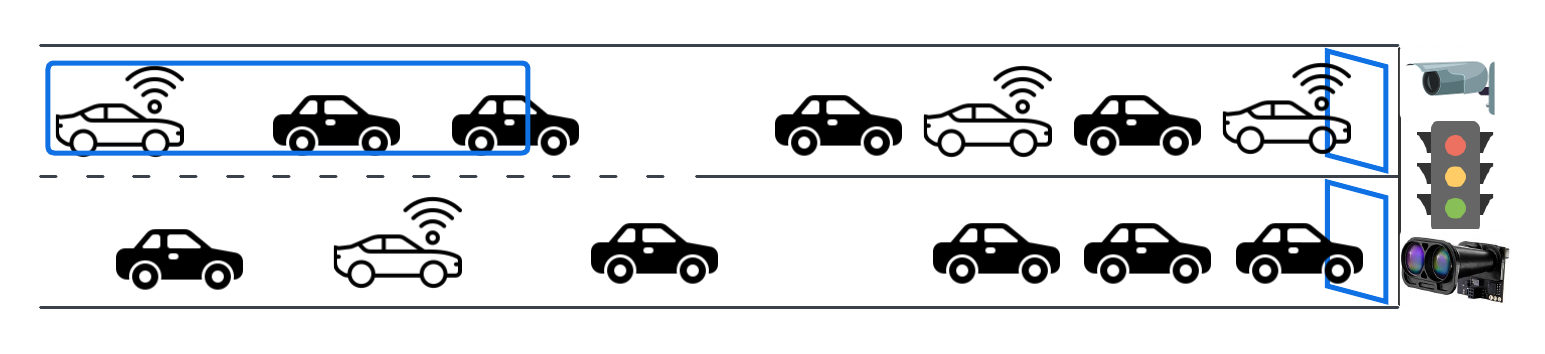
\includegraphics[width= 0.85\linewidth]{figures/sensors.png}
    \caption{Inductive loop detector, Video detection system, LiDAR, Connected vehicles}
    \label{fig: Loop detector position}
\end{figure}

Although the measurement function module in the PF-SIQE is versatile and adaptable to various sensors, it is impractical to include all sensor types within the scope of this thesis. Therefore, to demonstrate the framework's scalability and adaptability, this thesis will focus on the integration of three types of loop detectors and in-car sensors as examples. Assumptions:
\begin{itemize}
    \item The measurement outputs of loop detector $ z_k^\text{loop}$ includes
    \begin{itemize}
        \item count $\tilde c_k$ (number of vehicles passing the loop detector during time step $k$) from the count loop (i.e. loop 1). 
        \item occupancy $\tilde o_k$ (yes/ no during time step $k$) from the occupancy loop (i.e. loop 2). 
        \item average speed $\tilde v_k$ [m/s] from the speed loop (i.e. loop 3).
    \end{itemize}
    \item the placement of the loop detector is also tunable in the model, allowing it to be set as a parameter to adjust detection location based on specific road configurations.
    \item The measurement outputs of in-car sensor $z_k^\text{GPS}$ is position $\tilde d_k^i$ [m]. The $\tilde d_k^i$ contains information on the position and the corresponding vehicle ID.
    %speed $\tilde v_k^i$ [m/s], the relative speed to the predecessor $\Delta \tilde v_k^i$ [m/s], the current gap to the predecessor $\tilde s_k^i$ [m], the acceleration $\tilde a_k^i$ [m/s$^2$], the relative acceleration to the predecessor $\Delta \tilde a_k^i$ [m/s$^2$]. 
    %\item Assume the measurements from different sensors are independent.
    \item Assume that all output quantities are measured directly, and their noises are independent.
\end{itemize}


%when a GPS position $\beta(x_k)$ is near the downstream of the loop detector, which validates that a vehicle has passed the loop detector. 
The measurement function $g_k(z_k, n_k^\text{m})$: 
\begin{equation}
    z_k = \begin{bmatrix}
\text{$\tilde d_k^i$} \\
\text{$\tilde c_k$} \\
\text{$\tilde o_k$} \\
\text{$\tilde v_k$} \\
\text{$\cdot \cdot \cdot$} \\
\end{bmatrix}
= \begin{bmatrix}
\text{$f^\text{GPS}(x_k, n_k^\text{GPS})$} \\
\text{$f^\text{loop 1}(x_k, n_k^\text{loop 1})$} \\
\text{$f^\text{loop 2}(x_k, n_k^\text{loop 2})$} \\
\text{$f^\text{loop 3}(x_k, n_k^\text{loop 3})$} \\
\text{$\cdot \cdot \cdot$} \\
\end{bmatrix}
\end{equation}

where
\begin{itemize}
    \item $z_k$  denotes the measurement at time step $k$.
    \item $\tilde d_k^i$ represents the observed position of the $i$-th vehicle from in-car GPS at time step $k$.
    \item $\tilde c_k$ denotes the observed vehicle count (i.e. number of vehicles passing loop 1) at time step $k$.
    \item $\tilde o_k$ represents the observed loop occupancy from loop 2 at time step $k$.
    \item $\tilde v_k$ is the observed vehicle speed from loop 3 at time step $k$.
    \item $f^\text{GPS}(x_k, n_k^\text{GPS})$ is the function that models the GPS measurement, which is dependent on the state $x_k$ and the GPS measurement noise $n_k^\text{GPS}$.
    \item $f^\text{loop 1}(x_k, n_k^\text{loop 1})$, $f^\text{loop 2}(x_k, n_k^\text{loop 2})$, $f^\text{loop 3}(x_k, n_k^\text{loop 3})$ are functions modeling different types of loop detectors' measurements at different locations, dependent on the state $x_k$ and their respective measurement noises $n_k^\text{loop 1}$, $n_k^\text{loop 2}$, $n_k^\text{loop 3}$.
    \item The ellipses ($\cdot \cdot \cdot$) indicate that there could be additional measurements from other sensors or further configurations.
    \item $n_k^\text{m}$ is the measurement noise term. In this thesis, $n_k^\text{m}$ indicates the measurement noise from all the considered detectors, i.e. $n_k^\text{GPS}$,  $n_k^\text{loop 1}$, $n_k^\text{loop 2}$, $n_k^\text{loop 3}$, all independent.
\end{itemize}

In this framework, the measurement function $g_k(z_k, n_k^\text{m})$ aggregates the outputs from multiple sensor types, each with its respective noise distribution, into a single measurement vector $z_k$ for use in the particle filter estimation process. This modularity ensures the flexibility and adaptability of the PF-SIQE framework to various real-world sensor configurations. Next, Section \ref{Roadside sensor measurement noise distribution} and Section \ref{Floatings sensor measurement noise distribution} will investigate the measurement noise distribution from roadside sensors and floating sensors, and write the probability distribution function $p(z_k | x_k)$.

\subsection{Roadside Sensor Measurement Noise Distribution}\label{Roadside sensor measurement noise distribution}
As discussed in Section \ref{Roadside Sensor (Eulerian Sensor)}, it is crucial of extracting measurement noise distribution from the accuracy information/specification. This section will construct discrete probability distribution from the actual manufacturer's requirements. 


%As previously mentioned, the measurement outputs of $\alpha_k$ include $k, c_k^{\text{in}}, v_k^{\text{in}}, c_k^{\text{out}}, v_k^{\text{out}}$. To calculate $p(\alpha_k | x_k)$ requires a thorough examination of the noise distribution associated with $c_k$ and $v_k$. Surprisingly, this information is mentioned in the manufacturer's requirements.

\begin{table}[htp]
\centering
\begin{tabular}{p{0.8\linewidth}}
\toprule
\textbf{Vehicle Counting Accuracy} \\
\midrule
The number of vehicles counted deviates, in 95\% of the cases, by a maximum of 2\% from the actual number when a group of 1,000 vehicles passes a counting point on a lane. \\
\bottomrule
\end{tabular}

\vspace{0.1cm}

\begin{tabular}{p{0.8\linewidth}}
\toprule
\textbf{Speed Measurement Accuracy (95\% of cases)} \\
\midrule
\begin{itemize}
    \item 10\% if the speed is $\leq$ 20 km/h;
    \item 3\% if the speed is $>$ 20 km/h and $\leq$ 60 km/h;
    \item 5\% if the speed is $>$ 60 km/h and $\leq$ 180 km/h;
    \item 10\% if the speed is $>$ 180 km/h and $<$ 250 km/h.
\end{itemize} \\
\bottomrule
\end{tabular}

\vspace{0.1cm}

\begin{tabular}{p{0.8\linewidth}}
\toprule
\textbf{Speed Measurement Accuracy (remaining 5\% of cases)} \\
\midrule
\begin{itemize}
    \item 20\% if the speed is $\leq$ 20 km/h;
    \item 6\% if the speed is $>$ 20 km/h and $\leq$ 60 km/h;
    \item 10\% if the speed is $>$ 60 km/h and $\leq$ 180 km/h;
    \item 20\% if the speed is $>$ 180 km/h and $<$ 250 km/h.
\end{itemize} \\
\bottomrule
\end{tabular}
\caption{Loop detector Specifications. Source: Rijkswaterstaat, the Netherlands; translated by Henk Taale; used with permission. }
    \label{Loop detector Specifications. Source: Henk Taale, used with permission}
\end{table}

\subsubsection{Measurement Noise Distribution for Vehicle Count $\tilde c_k$ from Loop 1}
The measurement function of $\tilde c_k$ considering noise:

\begin{equation}
    \tilde c_k = c_k + n_k^\text{loop 1}
\end{equation}
\begin{equation}
    n_k^\text{loop 1} = f(c_k)
\end{equation}

\begin{equation}\label{VehicleCounting}
c_k = \sum_{i} \mathbb{I}(d_{k}^i \geq d^{\text{loop 1}}) \cdot \mathbb{I}(d_{k-1}^i \leq d^{\text{loop 1}})
\end{equation}

Where:
\begin{itemize}
    \item \(\mathbb{I}(\cdot)\) is the indicator function, which is 1 if the condition inside is true, and 0 otherwise.
\end{itemize}


To calculate the vehicle count \(c_k\) at time step \(k\) using the states \(x_k\), consider the upstream end of loop 1 \(d^{\text{loop 1}}\) and the vehicle position \(d_k^i\) with state noise. The pseudocode for calculating vehicle counts at time step \(k\) is shown below (see Algorithm \ref{Vehicle Counting Algorithm}). This algorithm initializes the count, iterates through each vehicle's position, and checks if the vehicle's position at time step \(k\) is downstream of the loop's upstream end. If so, it calculates the vehicle's position at the previous time step \(k-1\). If the position at \(k-1\) is upstream of the loop's upstream end, the vehicle is counted as having passed through the loop, and the count is incremented.

\begin{algorithm}[htp]
\caption{Vehicle Counting Algorithm for Loop 1}\label{Vehicle Counting Algorithm}
\begin{algorithmic}[1]
    \State \textbf{Input:} $d^{\text{loop 1}}, d_{k}^i$
    \State \textbf{Output:} $c_k$
    \State \textbf{Initialize:} $c_k$ $\gets 0$
    \For{$i = 1$ \textbf{to} $N$}
    %\For{$d_{k}^i$ in vehicle positions at $k$}
        \If{$d_{k}^i \geq d^{\text{loop 1}}$}
            \State Calculate $ d_{k-1}^i$
            \If{$ d_{k-1}^i \leq d^{\text{loop 1}}$}
                \State $c_k$ $\gets$ $c_k$ + 1
            \EndIf
        \EndIf
    \EndFor
    \State \Return $c_k$
\end{algorithmic}
\end{algorithm}  


Refer to Table \ref{Loop detector Specifications. Source: Henk Taale, used with permission}, for 95\% of the groups of 1,000 vehicles passing the counting point, the number of vehicles counted will be between 980 and 1,020. Given this context, this thesis assumes a normally distributed error in the vehicle count measurements $\tilde c_k$, which infers that the deviation from the actual count follows a normal distribution with specific parameters.

In a normal distribution $\mathcal{N}(\mu,\sigma^2)$, approximately 95\% of the data lies within 1.96 standard deviations from the mean. Here, the range is from 980 to 1,020, which means:
\begin{equation}
    1,000 \pm 1.96 \sigma =1,000 \pm 20
\end{equation}
Solution: $\sigma = \frac{20}{1.96} \approx 10.2$, therefore, vehicle count noise $n_k^\text{loop 1} \sim \mathcal{N}(1,000, 10.2^2)$, if 1000 vehicles have passed the loop. 

Because in practice, near intersections, it is often unrealistic to have exactly 1,000 vehicles or multiples of 1,000 vehicles passing the loop detector, it becomes essential to understand the accuracy distribution for any number of vehicles passing through. Therefore, it is beneficial to generalize the parameters $\mu_n, \sigma_n$ of the normal distribution based on $n$ vehicles. In this thesis, to be consistent and remove ambiguity, $n = c_k$. This enables the distribution to be applied more flexibly and accurately in a variety of practical scenarios.

%Given the context where the normal distribution \( \mathcal{N}(\mu, \sigma^2) \) for 1,000 vehicles has \(\mu = 1,000\) and \(\sigma \approx 10.2\), we can infer the corresponding parameters for \( n \) vehicles.

For \(c_k\) vehicles:
\begin{itemize}
    \item The mean \(\mu_{c_k}\) will be \(c_k\).
    \item The standard deviation \(\sigma_{c_k}\) can be scaled based on the standard deviation for 1,000 vehicles. Given that the standard deviation for 1,000 vehicles is 10.2, this thesis scales this based on the square root of \(c_k\).
\end{itemize}

The relationship between the standard deviation and the number of vehicles is given by:

\begin{equation}
    \sigma_{c_k} = 10.2 \times \sqrt{\frac{c_k}{1,000}}
\end{equation}

Thus, the normal distribution for \(c_k\) vehicles will be \( n_k^\text{loop 1} \sim \mathcal{N}(c_k, (10.2 \times \sqrt{\frac{c_k}{1,000}})^2) \), the probability distribution function will therefore be:

\begin{equation}\label{probability distribution loop 1}
    p^\text{loop 1}(\tilde c_k | c_k) = \frac{1}{\sqrt{2 \pi (10.2 \times \sqrt{\frac{c_k}{1,000}})^2}} \exp\left(-\frac{(\tilde c_k - c_k)^2}{2 (10.2 \times \sqrt{\frac{c_k}{1,000}})^2}\right)
\end{equation}

\subsubsection{Measurement Noise Distribution for Vehicle Presence $\tilde o_k$ from Loop 2}
The measurement function of $\tilde o_k$ considering noise:
\begin{equation}
    \tilde o_k = f(o_k, n_k^\text{loop 2})
\end{equation}

\begin{equation}\label{VehiclePresence}
o_k = \max \left( \mathbb{I}(d_{k}^i \geq d^{\text{loop 2}}) \cdot \mathbb{I}(d_{k-1}^i \leq d^{\text{loop 2}}) \right)
\end{equation}

Where:
\begin{itemize}
    \item \(\mathbb{I}(\cdot)\) is the indicator function, which is 1 if the condition inside is true, and 0 otherwise.
    \item The \(\max\) function ensures that \(o_k\) is set to 1 if any vehicle has crossed Loop 2 from time \(k-1\) to \(k\), exiting the loop as presence is detected.
\end{itemize}

To calculate the vehicle presence \(o_k\) at time step \(k\) using the states \(x_k\), consider the upstream end of loop 2 \(d^{\text{loop 2}}\) and the vehicle position \(d_k^i\) with state noise. Unlike the vehicle count \(c_k\), which can be greater than 1 within a single time step, the presence \(o_k\) is binary (either 1 or 0). If at least one vehicle passes through the loop within time step \(k\), \(o_k\) is set to 1 regardless of the number of vehicles.

It is important to note that accurate vehicle presence in time is crucial for detecting queues, as it provides essential information about how long a vehicle remains in the detection area. Misrepresentation of vehicle presence over time could lead to inaccurate queue detection, making it essential to address situations where the presence loop might not provide accurate results. The pseudocode for calculating vehicle presence at time step \(k\) is shown below (see Algorithm \ref{Vehicle Presence Algorithm}).


\begin{algorithm}[h]
\caption{Vehicle Presence Algorithm for Loop 2}\label{Vehicle Presence Algorithm}
\begin{algorithmic}[1]
    \State \textbf{Input:} $d^{\text{loop 2}}, d_{k}^i$
    \State \textbf{Output:} $o_k$
    \State \textbf{Initialize:} $o_k$ $\gets 0$
    \For{$i = 1$ \textbf{to} $N$}
    %\For{$d_{k}^i$ in vehicle positions at $k$}
        \If{$d_{k}^i \geq d^{\text{loop 2}}$}
            \State Calculate $d_{k-1}^i$
            \If{$d_{k-1}^i \leq d^{\text{loop 2}}$}
                \State $o_k$ $\gets$ 1
                \State \textbf{break} \Comment{Exit the loop as presence is detected}
            \EndIf
        \EndIf
    \EndFor
    \State \Return $o_k$
\end{algorithmic}
\end{algorithm}

This algorithm initializes the presence to 0, iterates through each vehicle's position, checks if the vehicle's position at time step \(k\) is downstream of the loop's upstream end, and if so, calculates the vehicle's position at the previous time step \(k-1\). If the position at \(k-1\) is upstream of the loop's upstream end, the presence is set to 1 and the loop is exited immediately, as detecting the presence of any vehicle is sufficient.

In Table \ref{Loop detector Specifications. Source: Henk Taale, used with permission}, there is no specific information provided for the presence detection accuracy of loop detectors. Therefore, this thesis assumes that the accuracy of vehicle presence detection is \( p \), meaning the probability that the measurement is correct is \( p \).

To model this, generate a random value \( r \sim \mathcal{U}[0,1] \). The vehicle presence measurement \( \tilde o_k \) is determined as follows:
\begin{itemize}
    \item If \( r < p \), then \( \tilde o_k \) is correct (i.e., matches the true vehicle presence \( o_k \)).
    \item If \( r \geq p \), then \( \tilde o_k \) is incorrect (i.e., does not match the true vehicle presence \( o_k \)).
\end{itemize}
The probability distribution function for vehicle presence \( \tilde o_k \) can be expressed as:

\begin{equation}\label{probability distribution function loop 2}
    p^\text{loop 2}(\tilde o_k | o_k) = 
    \begin{cases} 
        p, & \text{if } \tilde o_k = o_k \\
        1 - p, & \text{if } \tilde o_k \neq o_k
    \end{cases}
\end{equation}
Where the accuracy \( p \) is adjustable based on the specifications provided by different presence loop detector manufacturers.

\subsubsection{Measurement Noise Distribution for Vehicle Speed $\tilde v_k$ from Loop 3}

The measurement function for vehicle speed \( \tilde v_k \), considering noise, can be expressed as:
\begin{equation}
    \tilde v_k = v_k + n_k^\text{loop 3}
\end{equation}
\begin{equation}
    n_k^\text{loop 3} = f(v_k)
\end{equation}
To calculate the average speed \( v_k \) of the vehicles passing loop 3 (speed loop) during time step \( k \), it is essential to identify which vehicles have passed loop 3. This step is necessary because the average speed calculation relies on determining the vehicles that are physically crossing the loop during the time step, ensuring that the measured speed reflects only the vehicles interacting with the detector at that specific moment. Without identifying these vehicles, the calculated average speed could include vehicles that have not yet reached or have already passed the detector, leading to inaccurate results. This can be done by checking the position of each vehicle at time step \( k \) and the previous time step \( k-1 \). If the \( i^\text{th} \) vehicle's position at time step \( k \) is downstream of the loop 3's upstream end (\( d_{k}^i \geq d^{\text{loop 3}} \)) and its position at time step \( k-1 \) is upstream of the loop 3's upstream end (\( d_{k-1}^i \leq d^{\text{loop 3}} \)), then the \( i^\text{th} \) vehicle is identified as having passed loop 3. The average speed of all the vehicles passing loop 3 at time step \( k \) is then calculated as follows:



\begin{equation}\label{AverageSpeed}
v_k = 
\begin{cases}
\frac{\sum_{i} v_{k}^i \cdot \mathbb{I}(d_{k}^i \geq d^{\text{loop 3}}) \cdot \mathbb{I}(d_{k-1}^i \leq d^{\text{loop 3}})}{\sum_{i} \mathbb{I}(d_{k}^i \geq d^{\text{loop 3}}) \cdot \mathbb{I}(d_{k-1}^i \leq d^{\text{loop 3}})}, & \text{if } \sum_{i} \mathbb{I}(d_{k}^i \geq d^{\text{loop 3}}) \cdot \mathbb{I}(d_{k-1}^i \leq d^{\text{loop 3}}) > 0 \\
0, & \text{otherwise}
\end{cases}
\end{equation}

Where:
\begin{itemize}
    \item \(\mathbb{I}(\cdot)\) is the indicator function, which is 1 if the condition inside is true, and 0 otherwise.
    \item The numerator \(\sum_{i} v_{k}^i \cdot \mathbb{I}(d_{k}^i \geq d^{\text{loop 3}}) \cdot \mathbb{I}(d_{k-1}^i \leq d^{\text{loop 3}})\) sums the speeds of vehicles that have just passed Loop 3.
    \item The denominator \(\sum_{i} \mathbb{I}(d_{k}^i \geq d^{\text{loop 3}}) \cdot \mathbb{I}(d_{k-1}^i \leq d^{\text{loop 3}})\) counts the number of vehicles that have just passed Loop 3.
    \item If no vehicles have passed Loop 3, \(v_k\) is set to 0.
\end{itemize}



The pseudocode for these steps is shown in Algorithm \ref{Average Speed Calculation for Loop 3} below.
\begin{algorithm}[h]
\caption{Average Speed Calculation for Loop 3}\label{Average Speed Calculation for Loop 3}
\begin{algorithmic}[1]
    \State \textbf{Input:} $d^{\text{loop 3}}, d_{k}^i, v_{k}^i$
    \State \textbf{Output:} $v_k$
    \State \textbf{Initialize:} $v_k$ $\gets 0$
    \State \textbf{Initialize:} $n$ $\gets 0$ \Comment{Counter for vehicles passing the loop}
    \For{$i = 1$ \textbf{to} $N$}
    %\For{$d_{k}^i, v_{k}^i$ in vehicle positions and speeds at $k$}
        \If{$d_{k}^i \geq d^{\text{loop 3}}$}
            \State Calculate $d_{k-1}^i$
            \If{$d_{k-1}^i \leq d^{\text{loop 3}}$}
                \State $v_k \gets v_k + v_{k}^i$
                \State $n \gets n + 1$
            \EndIf
        \EndIf
    \EndFor
    \If{$n > 0$}
        \State $v_k \gets \frac{v_k}{n}$
    \Else
        \State $v_k \gets 0$ \Comment{No vehicles passed the loop}
    \EndIf
    \State \Return $v_k$
\end{algorithmic}
\end{algorithm}





In Table \ref{Loop detector Specifications. Source: Henk Taale, used with permission}, 95\% of the speed measurements fall within a specific accuracy range, and the remaining 5\% fall within a larger error range. 

For 95\% of the measured speeds, the accuracy is determined as follows:
\begin{equation}\label{speed loop noise1}
n_k^\text{loop 3} \sim 
\begin{cases}
\mathcal{U}[-0.1 v_k, 0.1 v_k], & \text{if  \( v_k \leq 20 \) km/h (i.e. \( v_k \leq 5.6 \) m/s)}, \\
\mathcal{U}[-0.03 v_k, 0.03 v_k], & \text{if \( 20 < v_k \leq 60 \) km/h (i.e. \( 5.6 < v_k \leq 16.7 \) m/s)}, \\
\mathcal{U}[-0.05 v_k, 0.05 v_k], & \text{if \( 60 < v_k \leq 180 \) km/h (i.e. \( 16.7 < v_k \leq 50 \) m/s)}, \\
\mathcal{U}[-0.1 v_k, 0.1 v_k], & \text{if \( 180 < v_k < 250 \) km/h (i.e. \( 50 < v_k < 69.4 \) m/s)}.
\end{cases}
\end{equation}

For the remaining 5\% of the measured speeds, the accuracy is at maximum twice as large:
\begin{equation}\label{speed loop noise2}
n_k^\text{loop 3} \sim 
\begin{cases}
\mathcal{U}[-0.2 v_k, 0.2 v_k], & \text{if } v_k \leq 20 \text{ km/h (i.e. } v_k \leq 5.6 \text{ m/s)}, \\
\mathcal{U}[-0.06 v_k, 0.06 v_k], & \text{if } 20 < v_k \leq 60 \text{ km/h (i.e. } 5.6 < v_k \leq 16.7 \text{ m/s)}, \\
\mathcal{U}[-0.1 v_k, 0.1 v_k], & \text{if } 60 < v_k \leq 180 \text{ km/h (i.e. } 16.7 < v_k \leq 50 \text{ m/s)}, \\
\mathcal{U}[-0.2 v_k, 0.2 v_k], & \text{if } 180 < v_k < 250 \text{ km/h (i.e. } 50 < v_k < 69.4 \text{ m/s)}.
\end{cases}
\end{equation}

The probability distribution function for vehicle speed \( \tilde v_k \) can be expressed as:
\begin{equation}
    p^\text{loop 3}(\tilde{v}_k | v_k) = 
    \begin{cases}
        \frac{0.95}{0.2 v_k}, & \text{for } 0.9 v_k \leq \tilde{v}_k \leq 1.1 v_k, v_k \leq 5.6 \text{ m/s,}  \\
        \frac{0.05}{0.4 v_k}, & \text{for } (0.8 v_k \leq \tilde{v}_k < 0.9 v_k \text{ or } 1.1 v_k < \tilde{v}_k \leq 1.2 v_k), v_k \leq 5.6 \text{ m/s,} \\
        \frac{0.95}{0.06 v_k}, & \text{for } 0.97 v_k \leq \tilde{v}_k \leq 1.03 v_k, 5.6 < v_k \leq 16.7 \text{ m/s,} \\
        \frac{0.05}{0.12 v_k}, & \text{for } (0.94 v_k \leq \tilde{v}_k < 0.97 v_k \text{ or } 1.03 v_k < \tilde{v}_k \leq 1.06 v_k), 5.6 < v_k \leq 16.7 \text{ m/s,} \\
        \frac{0.95}{0.1 v_k}, & \text{for } 0.95 v_k \leq \tilde{v}_k \leq 1.05 v_k, 16.7 < v_k \leq 50 \text{ m/s,} \\
        \frac{0.05}{0.2 v_k}, & \text{for } (0.9 v_k \leq \tilde{v}_k < 0.95 v_k \text{ or } 1.05 v_k < \tilde{v}_k \leq 1.1 v_k), 16.7 < v_k \leq 50 \text{ m/s,} \\
        \frac{0.95}{0.2 v_k}, & \text{for } 0.9 v_k \leq \tilde{v}_k \leq 1.1 v_k, 50 < v_k < 69.4 \text{ m/s,} \\
        \frac{0.05}{0.4 v_k}, & \text{for } (0.8 v_k \leq \tilde{v}_k < 0.9 v_k \text{ or } 1.1 v_k < \tilde{v}_k \leq 1.2 v_k), 50 < v_k < 69.4 \text{ m/s,} \\
        0, & \text{otherwise}.
    \end{cases}
\end{equation}





\subsubsection{Probability Distribution Function of Measurement Noise}
\begin{equation}\label{loop probability}
p(z_k^\text{loop}| x_k) = p^\text{loop 1}(\tilde c_k | c_k) \cdot p^\text{loop 2}(\tilde o_k | o_k) \cdot p^\text{loop 3}(\tilde v_k | v_k)
\end{equation}




\subsection{Floatings Sensor Measurement Noise Distribution}\label{Floatings sensor measurement noise distribution}
Section \ref{Global Positioning System (GPS)} has presented the noise characteristics of GPS data. For simplification, this thesis assumes that the measurement output from the GPS is directly \(\tilde d_k\) instead of latitude, longitude, and altitude. The mean and variance of the Gaussian noise distribution are assumed to be \( n_k^\text{GPS} \sim \mathcal{N}(\mu, \sigma^2) \). Typical standard deviations for civilian GPS horizontal position accuracy, with good satellite visibility, are around 3-10 meters. This thesis assumes $\mu = d_k$, \(\sigma = \sigma_\text{GPS}\) meters, resulting in \( n_k^\text{GPS} \sim \mathcal{N}(d_k, {\sigma_\text{GPS}}^2) \).

Thus, the measurement function for vehicle position \( \tilde d_k \), considering noise, can be expressed as:
\begin{equation}
    \tilde d_k = d_k + n_k^\text{GPS}
\end{equation}
\begin{equation}\label{gps noise}
    n_k^\text{GPS} = f(d_k) 
\end{equation}
The probability distribution function for vehicle position \( \tilde d_k \) can be expressed as:
\begin{equation}
    p^\text{GPS}(\tilde d_k | d_k) = \frac{1}{\sqrt{2\pi {\sigma_\text{GPS}}^2}} \exp\left(-\frac{(\tilde d_k - d_k)^2}{2{\sigma_\text{GPS}}^2}\right)
\end{equation}
%Given $\sigma = 5$, substituting the value into the equation gives:
%\begin{equation}
%p(\tilde d_k | d_k) = \frac{1}{\sqrt{2\pi \cdot 25}} \exp\left(-\frac{(\tilde d_k - d_k)^2}{2 \cdot 25}\right)
%\end{equation}

As noted in Section \ref{MF}, assume that the measurement outputs of \( z_k^\text{GPS} \) are all directly measured and their noises are independent. If additional sensor measurements are required, simply combine their independent probabilities by taking the product:
\begin{equation}\label{gps probability}
    p(z_k^\text{GPS} | x_k) = p(\tilde d_k | d_k) \cdot \cdot \cdot \cdot
\end{equation}

\subsection{Handling Multiple Vehicles}
To cope with multiple vehicles, the following assumptions are made:
\begin{itemize}
    \item The number of vehicles at time step $k$ is known.
    \item The GPS data for each vehicle is identifiable, meaning it is known which GPS position corresponds to which vehicle, even if the GPS positions are not accurate and cannot be matched perfectly with the vehicle.
\end{itemize}
The system measurement vector \( Z_k \) is extended to include the measurement vectors of all vehicles in every time step $k$:
\begin{equation}\label{system measurement vector}
    Z_k = \begin{bmatrix}
z_k^\text{GPS} \\
z_k^\text{loop}\\
\end{bmatrix}
= \begin{bmatrix}
z_k^1 \\
z_k^2 \\
\cdots \\
z_k^N \\
z_k^\text{loop 1}\\
z_k^\text{loop 2}\\
z_k^\text{loop 3}\\
\end{bmatrix}
= \begin{bmatrix}
\tilde d_k^1 \\
\tilde d_k^2 \\ 
\text{$\cdot \cdot \cdot $} \\
\tilde d_k^N \\ 
\tilde c_k  \\
\tilde o_k  \\
\tilde v_k  \\
\end{bmatrix}
= \begin{bmatrix}
 d_k^1 + n_k^\text{GPS}  \\ 
 d_k^2 + n_k^\text{GPS}  \\ 
\text{$\cdot \cdot \cdot $} \\
 d_k^N + n_k^\text{GPS}  \\
 c_k + n_k^\text{loop 1} \\
 f(o_k + n_k^\text{loop 2}) \\
 v_k + n_k^\text{loop 3} \\
\end{bmatrix}
\end{equation}

where \( N \) is the total number of vehicles.

\subsection{Probability Distribution Function of Measurement Noise}
In conclusion, $p(z_k | x_k)$ denotes the joint probability, derived by taking the product of $p(\tilde d_k | d_k)$, $p(\tilde c_k | c_k)$, $p(\tilde o_k | o_k)$ and $p(\tilde v_k | v_k)$. This product yields the probability of simultaneously observing the specific measurements from both the loop detectors and the in-car sensor, given the actual variables. 

Above all, the probability distribution function of measurement noise is:
\begin{equation}
    p(z_k | x_k) = \prod_{i=1}^{n^\text{loop}} p(z_k^\text{loop}| x_k)
   \cdot \prod_{i=1}^{n^\text{GPS}} p(z_k^\text{GPS} | x_k)
\end{equation}
where
\begin{itemize}
    \item $n^\text{loop}$ is the number of measurement outputs from detector loops.
    \item $n^\text{GPS}$ is the number of measurement outputs from GPS.
    \item $p(z_k^\text{loop}| x_k)$ is refer to Equation \ref{loop probability}.
    \item $p(z_k^\text{GPS} | x_k)$ is refer to Equation \ref{gps probability}.
\end{itemize}

\section{Estimation Outputs}
In line with the architecture of PF-SIQE shown in Figure \ref{PF-SIQE Architecture}, the direct output of PF-SIQE is the state estimate. Additionally, the queue estimate can be derived from the state estimate. This section will present both the state estimates and the queue estimates.
\subsection{State Estimates}
The state estimations output from the PF-SIQE are given by:
\begin{equation}\label{state estimates}
   \hat{e}_k^i = \begin{bmatrix}
\hat{d}_k^i & \hat{v}_k^i & \hat{a}_k^i & \hat{D}_k^i  
\end{bmatrix}
\end{equation}
where
\begin{itemize}
    \item $\hat{e}_k^i$ is the state estimations output of one vehicle.
    \item \(\hat{d}_k^i\) [m] is the estimated longitudinal position at time step \(k\).
    \item \(\hat{v}_k^i\) [m/s] is the estimated instantaneous speed at time step \(k\).
    \item \(\hat{a}_k^i\) [m/s$^2$]is the estimated instantaneous acceleration at time step \(k\).
    \item $\hat{D}_k^i$ is the decision of stop or go when facing the traffic light at time step \(k\).
\end{itemize}
The state estimations output vector \( E_k \) of multiple vehicles in every time step $k$:
\begin{equation}
    E_k = \begin{bmatrix}
\hat e_k^1 \\
\hat e_k^2 \\
\cdots \\
\hat e_k^N 
\end{bmatrix}
= \begin{bmatrix}
\hat{d}_k^1 & \hat{v}_k^1 & \hat{a}_k^1 & \hat{D}_k^1 \\
\hat{d}_k^2 & \hat{v}_k^2 & \hat{a}_k^2 & \hat{D}_k^2 \\
\text{$\cdot \cdot \cdot $} \\
\hat{d}_k^N & \hat{v}_k^N & \hat{a}_k^N & \hat{D}_k^N \\
\end{bmatrix}
\end{equation}

where \( N \) is the total number of vehicles.

\subsection{Queue Estimates}
In this thesis, the queue estimate is represented by the number of vehicles, \(\hat{n}_k\). Typically, this number can be used for signal control. A threshold speed, \(v_\text{threshold}\), is introduced as a parameter:
\begin{equation}\label{Queue Estimates}
\hat{n}_k = \sum_{i} \mathbb{I}(\hat{v}_{k}^i \leq v_\text{threshold})  
\end{equation}

Where:
\begin{itemize}
    \item \(\mathbb{I}(\cdot)\) is the indicator function, which is 1 if the condition inside is true, and 0 otherwise.
    \item \(v_\text{threshold}\) [m/s] is the threshold speed used to differentiate between stationary and moving vehicles.
\end{itemize}

In words, the equation sums up the number of vehicles whose estimated speeds $\hat v_k^i$ at time \(k\) are less than or equal to \(v_\text{threshold}\). By adjusting \(v_\text{threshold}\), the queue estimate can either reflect the number of stationary vehicles or the total number of vehicles that moving below a certain speed, providing flexibility in the estimation process.

\section{Summary}
This chapter has outlined the architecture and operational framework of the Particle Filter-Based Signalized Intersection Queue Estimator (PF-SIQE), focusing on the key modules: the state transition function module and the measurement function module. While the architecture and particle filter algorithm were introduced, the primary focus was on demonstrating the scalability and flexibility of the state transition and measurement function modules.

The state transition function module is highly adaptable and can be extended by integrating various microscopic traffic flow models, including lateral motion models. This flexibility ensures that future work can incorporate more complex vehicle behaviors beyond the longitudinal movements discussed in this thesis. Furthermore, the transition from estimating the state of a single vehicle to multiple vehicles is achieved by extending the state vector to a matrix format, accommodating a larger traffic flow within the studied road segment. It is important to note that the number of vehicles is assumed to remain constant within the segment during the analysis period, and this assumption will be further discussed in the final chapter.

The measurement function module similarly offers scalability, as it can accommodate a wide variety of detection technologies beyond the loop detectors utilized in this study. For instance, connected vehicle data or floating sensor measurements can easily be integrated into the model, enhancing its real-time applicability and accuracy.

Lastly, while this chapter has laid the groundwork for queue length estimation, the actual execution of simulations and validation of the model’s outputs, including queue estimates, will be presented in subsequent chapters. However, due to time constraints, the full implementation of queue estimation was not completed for simulation in this thesis, and the specific definition of the queue will be discussed in the final chapter, alongside recommendations for future work.







\begin{comment}
%According to the manufacturer’s requirements, for traffic management purposes, When a group of 1,000 vehicles passes a counting point, in 95\% of cases the number recorded deviates by no more than 2\% from the actual number of vehicles present. 

%it is feasible to develop a discrete noise distribution for the occupancy $\tilde c_k$. 



%Speed measurement accuracy for these vehicles is also maintained within precise margins, depending on the speed range. For speeds up to 20 km/h, the accuracy is determined within a 10\% margin 95\% of the time. As speeds increase beyond 20 km/h and up to 60 km/h, the accuracy tightens impressively to within 3\%. For vehicles traveling over 60 km/h and up to 180 km/h, measurements are 95\% accurate within a 5\% margin. However, for very high speeds ranging from 180 km/h to less than 250 km/h, the accuracy loosens back to a 10\% margin.

%In cases where precision is lower covering the remaining 5\% of speed measurements the margin of error increases. It doubles to 20\% for speeds up to 20 km/h, to 6\% for speeds between 20 km/h and 60 km/h, to 10\% for speeds between 60 km/h and 180 km/h, and again to 20\% for speeds between 180 km/h and under 250 km/h.



%According to the manufacturer’s requirements, it is feasible to develop a discrete noise distribution for the occupancy $\tilde c_k$. 


%noise in loop detector measurements that matches the detailed description provided. This task presents various challenges. For instance, constructing an equivalent discrete probability distribution becomes complicated when there are fewer than 1,000 vehicles. Additionally, considering that the focus of this study is on urban intersections where speed limits are typically 50 km/h, one must consider the feasibility of adjusting the criteria by excluding the category for speeds over 60 km/h. This modification could simplify the application to more common urban traffic scenarios.

%In this thesis, a simplified version is considered with the following assumptions:

\end{comment}








